\documentclass[a4paper,twoside]{article}
\usepackage[T1]{fontenc}
\usepackage[bahasa]{babel}
\usepackage{graphicx}
\usepackage{graphics}
\usepackage{float}
\usepackage[cm]{fullpage}
\pagestyle{myheadings}
\usepackage{etoolbox}
\usepackage{setspace} 
\usepackage{lipsum}

% Custom packages
\usepackage[]{hyperref} % links
\usepackage{listings} % block comments
\usepackage{subcaption} % subfigure
\usepackage[table]{xcolor} % program codes
\usepackage{verbatim} % inline comments
\usepackage{xspace} % force space

\setlength{\headsep}{30pt}
\usepackage[inner=2cm,outer=2.5cm,top=2.5cm,bottom=2cm]{geometry} %margin
% \pagestyle{empty}

\makeatletter
\renewcommand{\@maketitle} {\begin{center} {\LARGE \textbf{ \textsc{\@title}} \par} \bigskip {\large \textbf{\textsc{\@author}} }\end{center} }
\renewcommand{\thispagestyle}[1]{}
\markright{\textbf{\textsc{Laporan Perkembangan Pengerjaan Skripsi\textemdash Sem. Genap 2021/2022}}}

\graphicspath{{./Gambar/}}% folder tempat gambar 
%untuk url dan link
\hypersetup{unicode=true,colorlinks=true,linkcolor=blue,citecolor=green,filecolor=magenta, urlcolor=cyan}

\onehalfspacing

\hyphenation{me-ngu-rangi}
\hyphenation{ma-sya-ra-kat}
\hyphenation{com-mand}
\hyphenation{com-mands}
\hyphenation{line}
\hyphenation{me-nam-pil-kan}
\hyphenation{pe-rang-kat}
\hyphenation{kom-pu-ter}
\hyphenation{per-ka-kas}
 
\begin{document}

\title{\@judultopik}
\author{\nama \textendash \@npm} 

%ISILAH DATA BERIKUT INI:
\newcommand{\nama}{Alfred Aprianto Liaunardi}
\newcommand{\@npm}{6181801014}
\newcommand{\tanggal}{07/06/2022} %Tanggal pembuatan dokumen
\newcommand{\@judultopik}{Perkakas Command Line KIRI} % Judul/topik anda
\newcommand{\kodetopik}{PAN5201}
\newcommand{\jumpemb}{1} % Jumlah pembimbing, 1 atau 2
\newcommand{\pembA}{Pascal Alfadian Nugroho, M.Comp.}
\newcommand{\pembB}{-}
\newcommand{\semesterPertama}{52 - Genap 21/22} % semester pertama kali topik diambil, angka 1 dimulai dari sem Ganjil 96/97
\newcommand{\lamaSkripsi}{1} % Jumlah semester untuk mengerjakan skripsi s.d. dokumen ini dibuat
\newcommand{\kulPertama}{Skripsi 1} % Kuliah dimana topik ini diambil pertama kali
\newcommand{\tipePR}{B} % tipe progress report :
% A : dokumen pendukung untuk pengambilan ke-2 di Skripsi 1
% B : dokumen untuk reviewer pada presentasi dan review Skripsi 1
% C : dokumen pendukung untuk pengambilan ke-2 di Skripsi 2

% New words/phrases
\newcommand{\chromewebstorecli}{Chrome \textit{Web Store Item Property} CLI\xspace}
\newcommand{\cl}{\textit{command line}\xspace}
\newcommand{\cli}{\textit{command line interface}\xspace}
\newcommand{\googlemapscli}{Google \textit{Maps Direction} CLI\xspace}
\newcommand{\gui}{\textit{graphical user interface}\xspace}
\newcommand{\itunesapi}{\textit{iTunes Search} API\xspace}
\newcommand{\latlon}{\textit{latitude} dan \textit{longitude}\xspace}
\newcommand{\logoregistered}{\textsuperscript{\textregistered}}
\newcommand{\logotrademark}{\textsuperscript{TM}}
\newcommand{\ubercli}{Uber CLI\xspace}

% Custom commands
\renewcommand{\refname}{\centering DAFTAR REFERENSI}
\lstset{numbers=left,stepnumber=1, numbersep=5pt, frame=single,frameround={tttt},
	tabsize=4, breaklines=true, basicstyle=\fontfamily{fvm}\selectfont\tiny, 
	commentstyle=\itshape\color{gray}, keywordstyle=\bfseries\color{blue}, 
	identifierstyle=\color{black}, stringstyle=\color{orange},
	literate={-}{-}1{-\,-}{--}1
} % lstlisting formatting

% Dokumen hasil template ini harus dicetak bolak-balik !!!!

\maketitle

\pagenumbering{arabic}

\section{Data Skripsi} %TIDAK PERLU MENGUBAH BAGIAN INI !!!
Pembimbing utama/tunggal: {\bf \pembA}\\
Pembimbing pendamping: {\bf \pembB}\\
Kode Topik : {\bf \kodetopik}\\
Topik ini sudah dikerjakan selama : {\bf \lamaSkripsi} semester\\
Pengambilan pertama kali topik ini pada : Semester {\bf \semesterPertama} \\
Pengambilan pertama kali topik ini di kuliah : {\bf \kulPertama} \\
Tipe Laporan : {\bf \tipePR} -
\ifdefstring{\tipePR}{A}{
			Dokumen pendukung untuk {\BF pengambilan ke-2 di Skripsi 1} }
		{
		\ifdefstring{\tipePR}{B} {
				Dokumen untuk reviewer pada presentasi dan {\bf review Skripsi 1}}
			{	Dokumen pendukung untuk {\bf pengambilan ke-2 di Skripsi 2}}
		}
		
\section{Latar Belakang}
\label{sec:label}
Project KIRI\footnote{\href{https://projectkiri.id}{https://projectkiri.id}} (akan disingkat sebagai KIRI dalam dokumen ini) adalah sebuah perangkat lunak berbasis web yang dibuat untuk \mbox{membantu} mengurangi efek dari kemacetan. KIRI mengurangi dampak kemacetan dengan membantu penggunanya, baik \mbox{masyarakat} maupun turis, dalam menggunakan salah satu sarana transportasi umum yang ada di Indonesia, yaitu angkutan kota (angkot). Cara KIRI \mbox{mempermudah} penggunaan angkot adalah dengan menunjukkan rute yang akan ditempuh, beserta langkah-langkah yang harus dilakukan oleh pengguna yang ingin bepergian dari satu titik ke titik lain, mulai dari seberapa jauh pengguna harus berjalan untuk menaiki angkot yang bersangkutan, di mana pengguna harus naik atau turun, seberapa jauh lagi pengguna harus berjalan sampai ke titik tujuan, dan seberapa lama estimasi waktu perjalanan yang akan ditempuh. Untuk kebutuhan pembuatan perangkat lunak yang memanfaatkan fitur dari KIRI, tersedia juga REST API KIRI yang dapat digunakan secara praktis. Adapun tampilan dari halaman web ini dapat dilihat di gambar \ref{fig:kiri-page}. 
\vspace{\baselineskip}
\begin{figure}[ht]
    \centering
    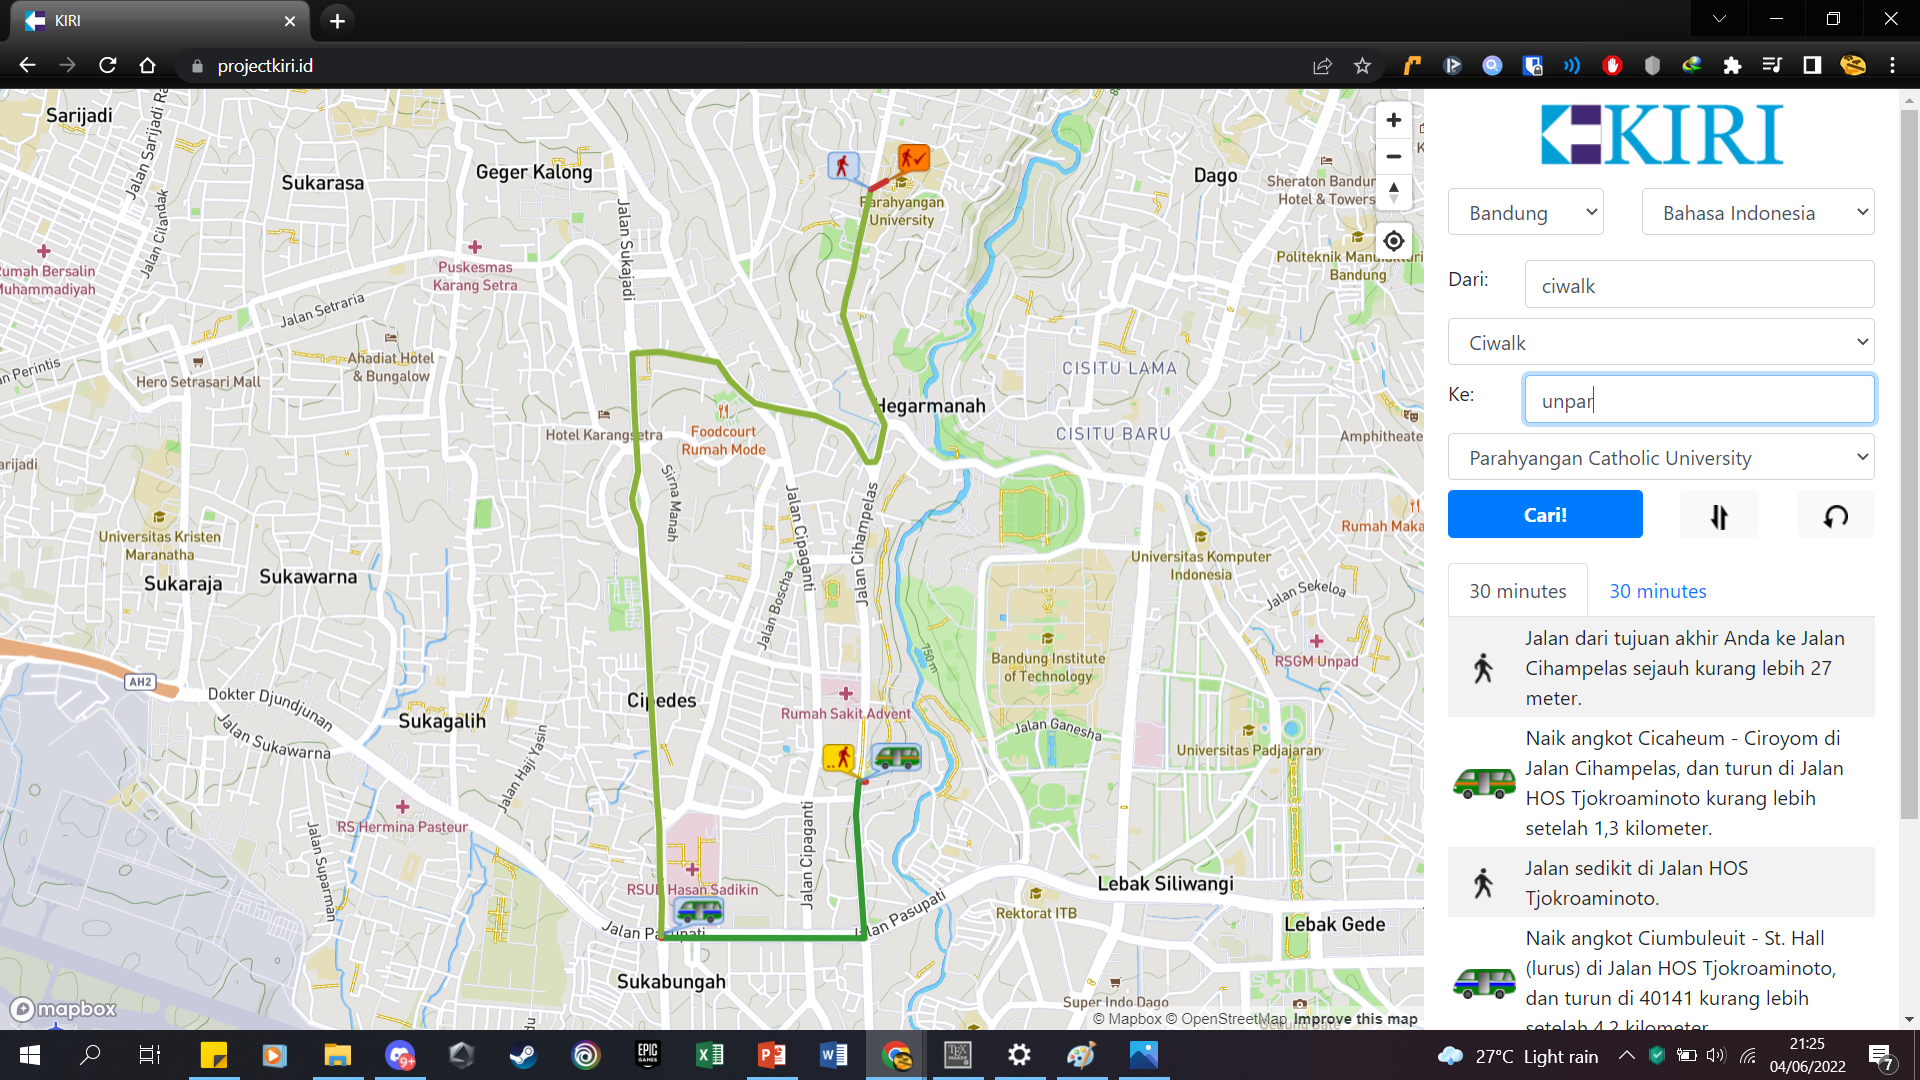
\includegraphics[width=0.74\linewidth]{projectkiri-example}
    \caption[Tampilan halaman web KIRI]{Tampilan halaman web KIRI, yang menunjukkan rute dari Cihampelas Walk ke Universitas Katolik Parahyangan.}
    \label{fig:kiri-page}
\end{figure}

\vfill\newpage
Sementara itu, dalam komputer, salah satu dari sekian banyak tipe perangkat lunak adalah perangkat lunak \textit{command line}. \textit{\mbox{Command} line} (\cl \textit{interpreter}, atau \cl \textit{interface}) adalah sebuah perangkat lunak berupa sebuah kotak/\textit{window} yang memuat teks berupa perintah-perintah,\footnote{\href{https://ubuntu.com/tutorials/command-line-for-beginners\#3-opening-a-terminal}{Ubuntu Tutorials - The Linux command line for beginners: 3. Opening a Terminal}} yang menerima masukan dari pengguna dan  menjalankannya.\cite{marsh:2010:fatfreeintrotocommandline} Perintah-perintah ini hanya berupa gabungan dari teks and simbol-simbol berupa karakter, tanpa ada tambahan gambar grafis apapun. Singkatnya, tipe perangkat lunak ini bukan merupakan tipe yang paling indah untuk dilihat oleh para pengguna, tetapi jika digunakan dengan tepat, maka \mbox{jenis} \mbox{perangkat} lunak ini bisa menyuruh komputer untuk melakukan banyak sekali perintah-perintah dengan sangat cepat dan sangat efektif.

Pada skripsi ini akan dibuat sebuah perangkat lunak berupa perkakas \cl (\textit{command line tool}) yang dapat menjalankan fungsi-fungsi API dari KIRI. Perangkat lunak ini, seperti jenisnya, akan dibuat murni sebagai perkakas yang dijalankan dari \cl (terminal, cmd, PowerShell, dll.), dan tampilan akhir dari perangkat lunak akan berupa \cli tanpa tambahan \textit{graphical user interface}. Keseluruhan dari perangkat lunak ini akan dibangun dalam bahasa C.

\section{Rumusan Masalah}
\label{sec:rumusan}
\begin{enumerate}
	\item Bagaimana membangun perkakas \textit{command line} yang dapat mengimplementasikan fitur-fitur API KIRI dalam bahasa C?
	\item Bagaimana integrasi perkakas \textit{command line} KIRI dapat dilakukan dengan perkakas-perkakas \textit{command line} lainnya di Linux?
\end{enumerate}

\section{Tujuan}
\label{sec:tujuan}
Batasan masalah dalam skripsi ini adalah sebagai berikut:
\begin{enumerate}
	\item Membangun perkakas \textit{command line} yang dapat mengimplementasikan fitur-fitur API KIRI dalam bahasa C.
	\item Melakukan integrasi perkakas \textit{command line} KIRI dengan perkakas-perkakas \textit{command line} lainnya di Linux.
\end{enumerate}

\section{Deskripsi Perangkat Lunak}
\label{sec:description}
Perangkat lunak akhir yang akan dibuat memiliki fitur minimal sebagai berikut:
\begin{itemize}
	\item Pengguna dapat memasukkan lokasi awal dan tujuan akhir sebagai masukan dari perangkat lunak.
	\item Pengguna dapat melihat langkah-langkah yang harus ditempuh dalam perjalanan, mulai dari angkot mana saja yang harus dinaiki, ke mana pengguna harus berjalan kaki untuk bisa mencapai angkot terdekat dari lokasi terakhir pengguna, sampai seberapa jauh pengguna harus berjalan untuk mencapai tujuan akhir.
	\item Pengguna dapat melihat jarak yang harus ditempuh untuk setiap langkahnya.
	\item Pengguna dapat melihat seberapa lama waktu perjalanan untuk setiap langkahnya.
\end{itemize}

\section{Detail Perkembangan Pengerjaan Skripsi}
\label{sec:devdetail}
Detail bagian pekerjaan skripsi sesuai dengan rencan kerja/laporan perkembangan terkahir :
	\begin{enumerate}
		\item \textbf{Melakukan eksplorasi fungsi-fungsi perangkat lunak KIRI serta eksplorasi cara \mbox{implementasi} API KIRI.}\\
		{\bf Status :} Ada sejak rencana kerja skripsi.\\
		{\bf Hasil :} KIRI merupakan sebuah perangkat lunak berbasis web yang berfungsi untuk menyelesaikan (atau setidaknya mengurangi) dampak dari masalah-masalah yang dapat diselesaikan oleh \mbox{transportasi} umum/publik di Indonesia, seperti pemanasan global, kemacetan, atau peningkatan harga bensin. \mbox{Selain} itu, turis mancanegara juga memilih untuk menaiki transportasi umum, karena jenis \mbox{sarana} transportasi tersebut tidak hanya jauh lebih murah, tetapi juga memberikan kesempatan yang \mbox{mudah} kepada mereka untuk melihat seluk-beluk dari kota-kota yang mereka kunjungi. Walaupun \mbox{begitu}, \mbox{banyak} masyarakat lokal sendiri yang seringkali masih segan untuk menaiki transportasi publik, umumnya karena transportasi publik dianggap lebih rumit persiapannya dibandingkan dengan metode-metode transportasi privat, seperti menaiki kendaraan pribadi.\footnote{\href{https://projectkiri.github.io/\#about-kiri}{https://projectkiri.github.io/\#about-kiri}}

Di halaman web KIRI, pengguna dapat memasukkan input berupa lokasi awal dan lokasi tujuan dan KIRI akan menghasilkan seluruh langkah yang harus ditempuh oleh pengguna untuk sampai ke lokasi tujuan, dengan menggunakan angkot. Keluaran ini sudah meliputi kode angkot mana saja yang harus dinaiki, dan juga seberapa jauh pengguna harus berjalan kaki untuk sampai ke lokasi rute angkot berikutnya.

KIRI memiliki sebuah API yang dapat digunakan untuk keperluan pengembangan perangkat \mbox{lunak}. API ini menyediakan tiga buah jenis layanan web (\textit{webservice}), yang ketiganya dapat dilakukan \mbox{dengan} mengirim permintaan (\textit{request}) tipe GET melalui API tersebut. Isi dari permintaan yang perlu \mbox{dikirimkan} serta respons dari API yang akan dikembalikan berbeda tergantung dari jenis layanan yang digunakan. Adapun ketiga jenis layanan tersebut adalah pencarian tempat (\textit{search place}), pencarian rute (\textit{routing}), dan \textit{smart direction}.

\vspace{\baselineskip}
\textbf{\textit{\large{Search Place}}}
\label{sec:kiri-api-searchplace}

Layanan pencarian lokasi (\textit{search place}) adalah layanan web pada API KIRI yang berfungsi untuk mencari suatu lokasi berdasarkan kata kunci yang diberikan oleh pengguna. Untuk menggunakan layanan ini, pengguna harus mengirim permintaan GET ke alamat \href{https://projectkiri.id/api}{https://projectkiri.id/api}. Adapun permintaan tersebut harus memiliki parameter-parameter seperti terlihat di bawah ini.

\begin{itemize}
	\item \verb|version|\\
	\textbf{Kemungkinan nilai:} \verb|2|\\
	Parameter ini merupakan tanda bagi API untuk menggunakan protokol versi 2.
	\item \verb|mode|\\
	\textbf{Kemungkinan nilai:} \verb|searchplace|\\
	Parameter ini merupakan mode dari servis/jasa API yang akan digunakan oleh pengguna. Untuk pengunaan layanan pencarian lokasi, variabel ini harus diisi dengan \verb|searchplace|.
	\item \verb|region|\\
	\textbf{Kemungkinan nilai:} \verb|cgk|, \verb|bdo|, \verb|mlg|, atau \verb|sub|\\
	Parameter ini merupakan kode bandara IATA tiga huruf yang merepresentasikan daerah mana tempat lokasi yang ingin dicari berada. Kode yang dapat diproses oleh API ini meliputi \verb|cgk| (Cengkareng/Jakarta), \verb|bdo| (Bandung), \verb|mlg| (Malang), dan \verb|sub| (Surabaya).
	\item \verb|querystring|\\
	\textbf{Kemungkinan nilai:} \textit{string} apapun dengan panjang minimal satu karakter\\
	Parameter ini berisi kata kunci yang akan digunakan untuk menentukan lokasi yang ingin dicari pengguna.
	\item \verb|apikey|\\
	\textbf{Kemungkinan nilai:} angka heksadesimal 16-digit\\
	Parameter ini berisi kunci API pribadi yang harus digenerasi terlebih dahulu sebelum API dapat digunakan.
\end{itemize}

Perlu diperhatikan bahwa salah satu dari parameter yang harus diikutkan dalam pesan tersebut merupakan parameter yang meminta kunci API. Kunci tersebut harus dibuat terlebih dahulu sebelum API KIRI dapat digunakan, melalui halaman \textit{API Keys} KIRI,\footnote{\href{https://projectkiri.id/dev/apikeys}{https://projectkiri.id/dev/apikeys}} yang dapat dilihat di gambar \ref{fig:kiri-apikeypage}. Untuk perkakas ini, kunci API ini akan bernilai \verb|68C...97C|.\footnote{Bagian tengah dari kunci API diganti dengan "..." untuk alasan keamanan.}

\begin{figure}[t]
    \centering
    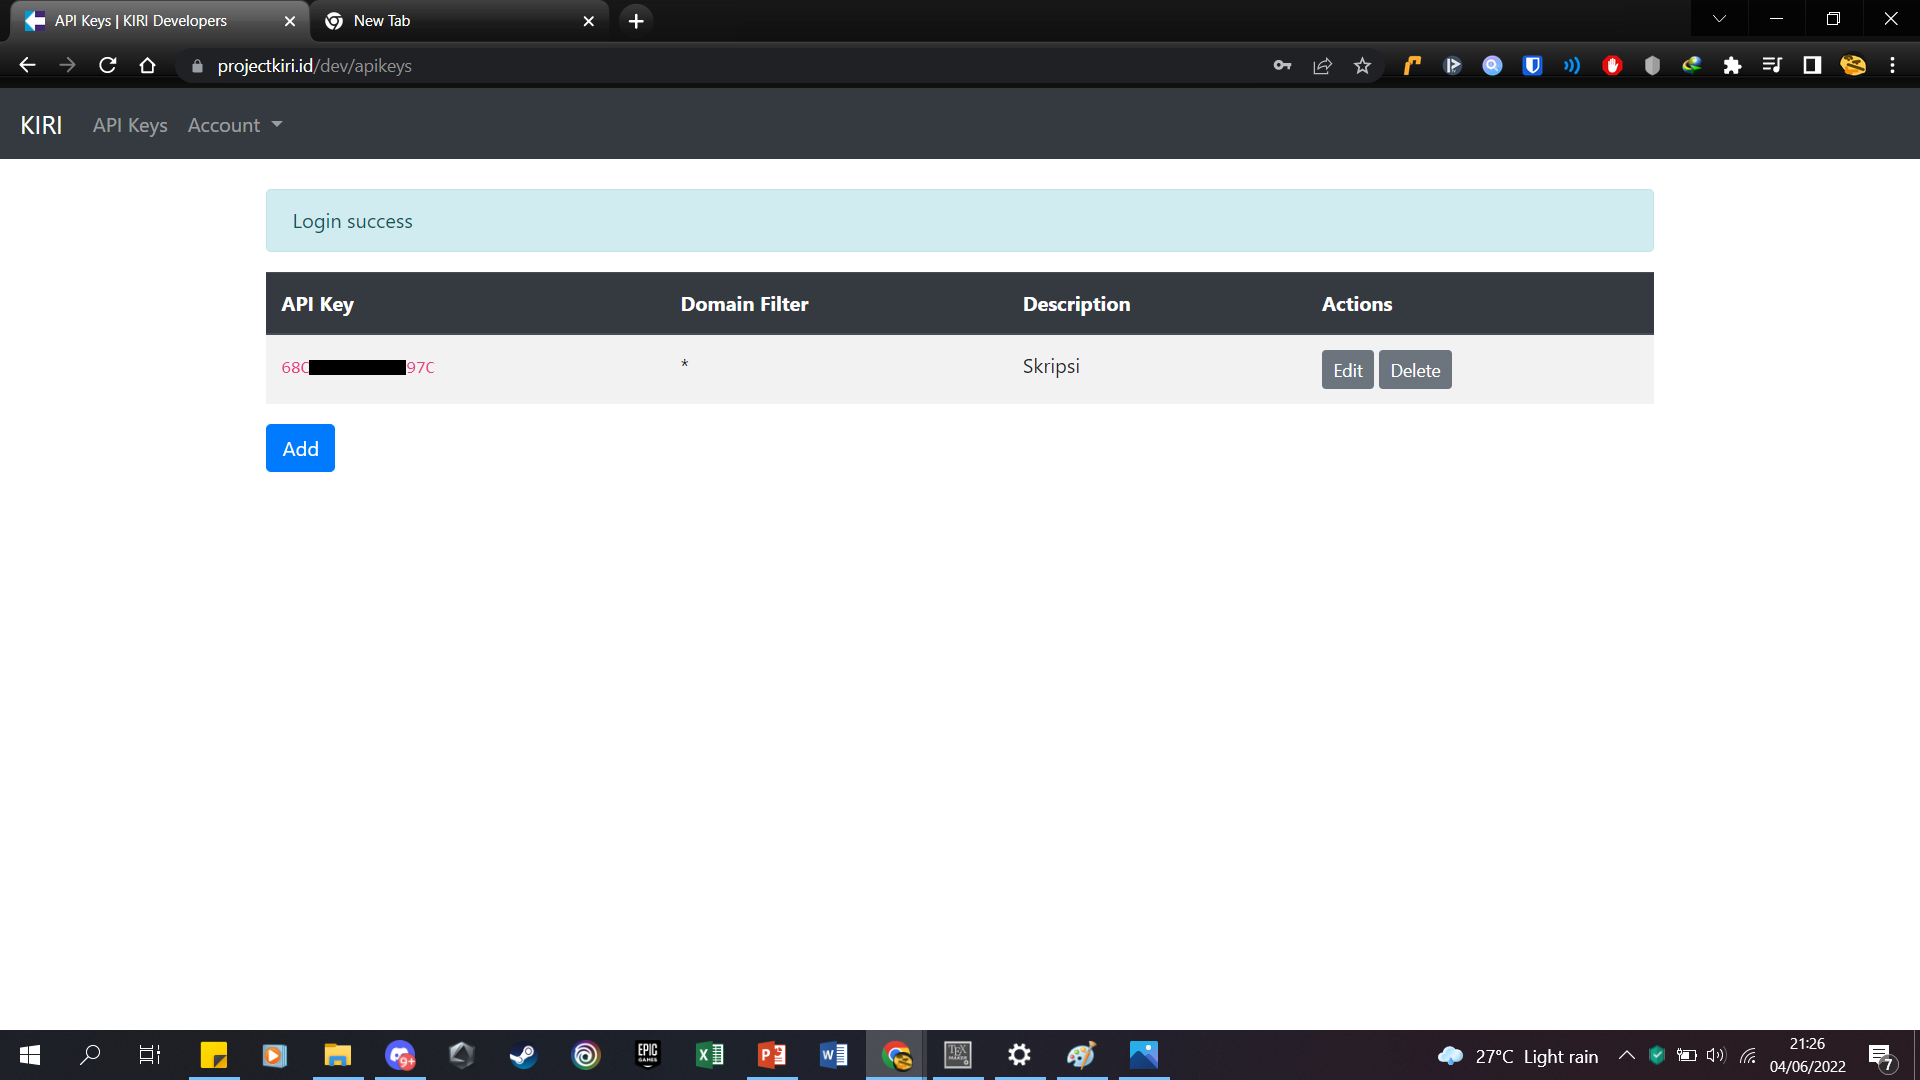
\includegraphics[width=0.75\linewidth]{projectkiri-apikey}
    \caption[Halaman web \textit{API Keys} KIRI.]{Halaman web \textit{API Keys} KIRI.}
    \label{fig:kiri-apikeypage}
\end{figure}

Untuk mengakses halaman tersebut, pengguna harus membuat sebuah akun terlebih dahulu. Ketika akun sudah dibuat, maka pengguna baru akan dapat membuat kunci API yang dibutuhkan, sekaligus membuat filter \textit{domain}, yang membatasi di \textit{domain} mana saja kunci tersebut dapat digunakan, serta memberikan deskripsi untuk kunci API tersebut. Kunci ini kemudian dapat digunakan sebagai nilai dari parameter \verb|apikey| yang diperlukan dalam permintaan tadi.

Sebelum membahas keluaran dari layanan API ini, perlu ditegaskan dulu apa definisi dari nilai \latlon suatu lokasi. \textit{Latitude} merupakan berapa derajat sebuah tempat berada dari garis ekuator, dengan lokasi-lokasi yang berada maksimum 90 derajat di atas ekuator memiliki nilai \textit{latitude} positif, sedangkan lokasi-lokasi yang berada maksimum 90 derajat di bawah ekuator memiliki nilai \textit{latitude} negatif. Sedangkan, \textit{longitude} merupakan berapa derajat lokasi sebuah tempat berada dari garis meridian (bujur) utama Bumi, dengan rentang nilai dari -180 derajat di sisi kiri (barat) meridian utama, hingga 180 derajat di kanan (timur) bujur tersebut.\footnote{\href{https://gsp.humboldt.edu/olm/Lessons/GIS/01\%20SphericalCoordinates/Latitude\_and\_Longitude.html}{https://gsp.humboldt.edu/olm/Lessons/GIS/01\%20SphericalCoordinates/Latitude\_and\_Longitude.html}} Kedua nilai ini merupakan salah satu dari dua variabel yang dikembalikan dalam respons API untuk layanan ini, dengan variabel lainnya berupa nama dari lokasi yang ditemukan itu sendiri. Adapun respons yang diberikan oleh API akan berupa sebuah objek JSON yang selalu memiliki setidaknya dua variabel, yaitu:
\vfill\newpage % prevent widow
\begin{itemize}
	\item \verb|status|\\
	\textbf{Kemungkinan nilai:} \verb|ok| atau \verb|error|\\
	Variabel ini menandakan apakah permintaan berhasil diproses atau tidak. Jika permintaan \mbox{berhasil} diproses, variabel ini akan bernilai \verb|ok|, dan jika tidak, variabel ini akan bernilai \verb|error|.
	\item \verb|searchresult|\\
	Variabel ini merupakan hasil pencarian yang ditemukan oleh layanan API ini. Isi dari variabel ini merupakan objek \textit{array} yang masing-masing memiliki variabel berikut:
	
	\begin{itemize}
		\item \verb|placename|\\
		Variabel ini berisi nama lokasi yang ditemukan berdasarkan kata kunci yang diberikan oleh pengguna.
		\item \verb|location|\\
		Variabel ini berisi nilai \latlon dari lokasi yang ditemukan dalam pencarian.
	\end{itemize}
	
\end{itemize}
\noindent
Contoh dari penggunaan API KIRI untuk layanan ini dapat dilihat di gambar \ref{fig:kiri-api-searchplace-usage}.

\begin{figure}[t]
    \centering
    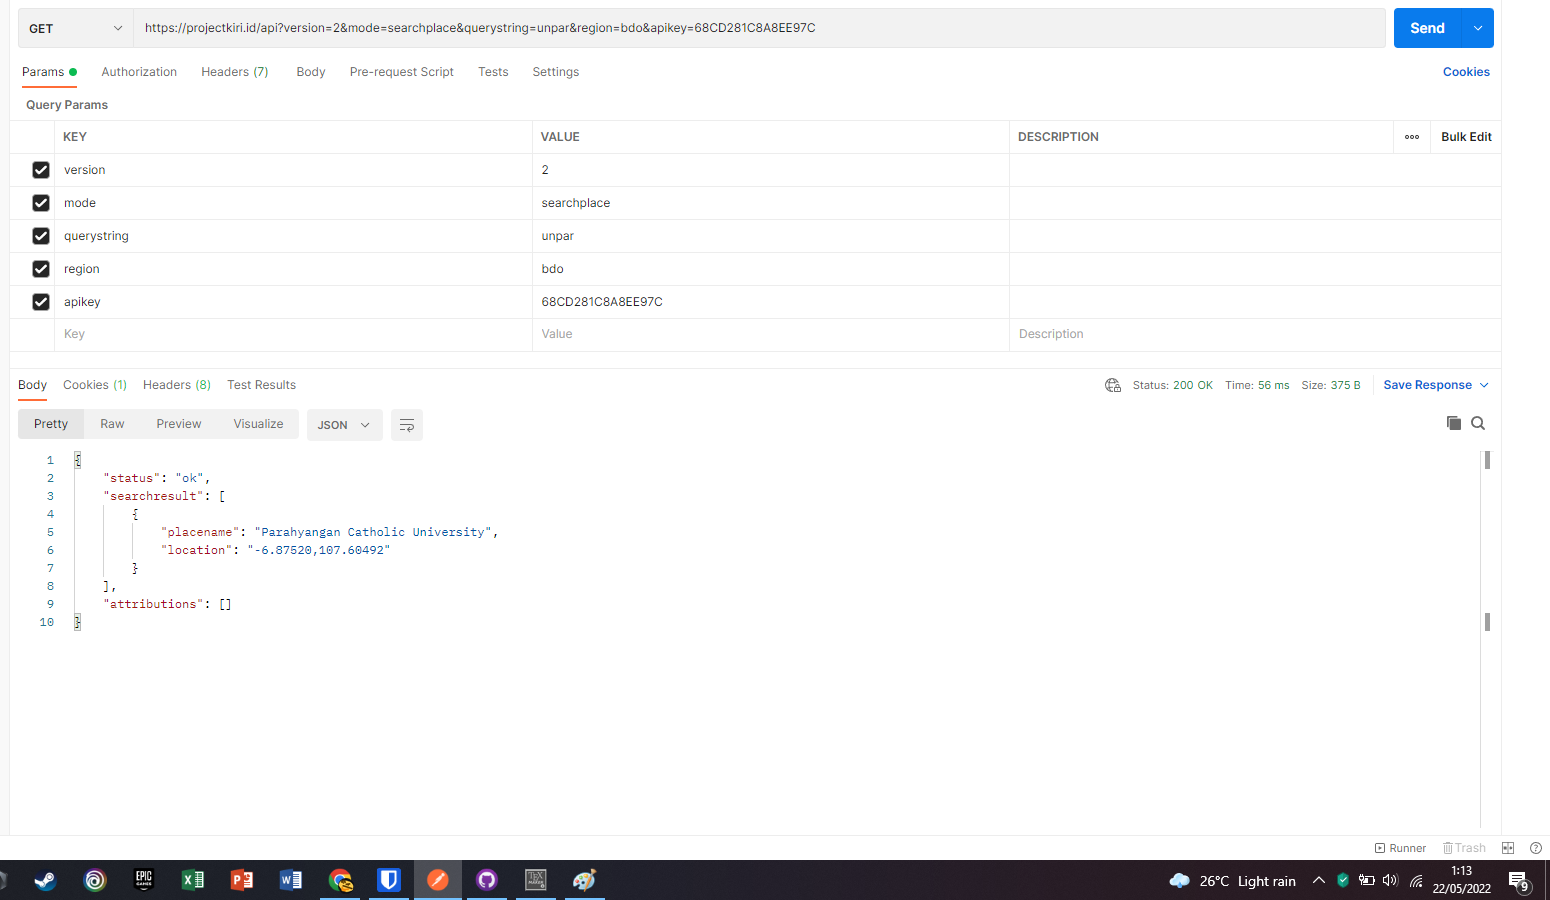
\includegraphics[width=0.74\linewidth]{apikiri-searchplace}
    \caption[Penggunaan API KIRI untuk layanan pencarian lokasi]{Penggunaan API KIRI untuk layanan pencarian lokasi menggunakan Postman. Gambar ini menunjukkan hasil pencarian lokasi ``unpar'' di daerah Bandung.}
    \label{fig:kiri-api-searchplace-usage}
\end{figure}

\vspace{\baselineskip}
\textbf{\textit{\large{Routing}}}
\label{sec:kiri-api-routing}

Layanan pencarian rute (\textit{routing}) adalah layanan web pada API KIRI yang memiliki fungsi yang sama dengan fungsi utama dari perangkat lunak KIRI sendiri, yaitu menunjukkan rute serta langkah-langkah yang harus ditempuh untuk pergi dari satu lokasi ke lokasi lainnya, dengan menggunakan angkot yang tersedia. Untuk menggunakan layanan ini, pengguna harus mengirim permintaan GET ke alamat \href{https://projectkiri.id/api}{https://projectkiri.id/api}. Adapun permintaan tersebut harus memiliki parameter-parameter seperti terlihat di bawah ini.

\begin{itemize}
	\item \verb|version|\\
	\textbf{Kemungkinan nilai:} \verb|2|\\
	Parameter ini merupakan tanda bagi API untuk menggunakan protokol versi 2.
	\item \verb|mode|\\
	\textbf{Kemungkinan nilai:} \verb|findroute|\\
	Parameter ini merupakan mode dari servis/jasa API yang akan digunakan oleh pengguna. Untuk pengunaan layanan pencarian rute dengan angkot, variabel ini diisi dengan \verb|findroute|.
	\item \verb|locale|\\
	\textbf{Kemungkinan nilai:} \verb|en| atau \verb|id|\\
	Parameter ini mengatur bahasa apa yang akan digunakan dalam keluaran API nantinya\textemdash\verb|en| berarti keluaran akan menggunakan bahasa Inggris, dan \verb|id| berarti keluaran akan menggunakan bahasa Indonesia.
	\item \verb|start|\\
	\textbf{Kemungkinan nilai:} \verb|lat|, \verb|lng|; dalam bentuk desimal\\
	Parameter ini merupakan nilai \latlon dari titik awal perjalanan pengguna.
	\item \verb|finish|\\
	\textbf{Kemungkinan nilai:} \verb|lat|, \verb|lng|; dalam bentuk desimal\\
	Parameter ini berisi nilai \latlon dari titik akhir/tujuan perjalanan pengguna.
	\item \verb|presentation| (opsional)\\
	\textbf{Kemungkinan nilai:} \verb|desktop|\\
	Parameter ini hanya digunakan untuk fitur \textit{backwards compatibility}.
	\item \verb|apikey|\\
	\textbf{Kemungkinan nilai:} angka heksadesimal 16-digit\\
	Parameter ini berisi kunci API pribadi yang harus digenerasi terlebih dahulu sebelum API dapat digunakan.
\end{itemize}
\vspace{\baselineskip}
Sedangkan, respons yang diberikan oleh API akan berupa sebuah objek JSON yang selalu memiliki setidaknya dua variabel, yaitu:

\begin{itemize}
	\item \verb|status|\\
	\textbf{Kemungkinan nilai:} \verb|ok| atau \verb|error|\\
	Variabel ini menandakan apakah permintaan berhasil diproses atau tidak. Jika permintaan \mbox{berhasil} diproses, variabel ini akan bernilai \verb|ok|, dan jika tidak, variabel ini akan bernilai \verb|error|.
	\item \verb|message|\\
	Variabel ini bisa berisi dua macam objek. Jika permintaan dari user tidak berhasil diproses, atau dalam kata lain, terjadi sebuah \textit{error}, maka variabel ini akan berisi string yang merupakan pesan \textit{error} serta alasan spesifik mengapa \textit{error} tersebut terjadi. Di lain sisi, jika permintaan dari user berhasil diproses, variabel ini akan mengalami dua perubahan utama. Pertama, nama variabel ini akan berubah menjadi \verb|routingresults|, dan kedua, isi dari variabel ini akan menjadi sebuah \textit{array} JSON yang merupakan respons dari API KIRI berupa keluaran yang akan dilihat oleh pengguna. \textit{Array} JSON ini sendiri terbagi menjadi beberapa variabel lainnya, yang dapat dilihat di daftar di bawah ini.
	
	\begin{itemize}
		\item \verb|steps|\\
		\textbf{Tipe:} \textit{array}\\
		Variabel ini merepresentasikan satu buah langkah yang harus ditempuh oleh pengguna. Adapun \textit{array} ini sendiri berisi variabel-variabel berikut:
		
		\begin{itemize}
			\item Tipe transportasi\\
			Tipe sarana transportasi yang harus dipakai oleh pengguna. Jika pengguna harus berjalan kaki, variabel ini akan berisi \verb|walk|. Jika pengguna harus menaiki angkot, variabel ini akan berisi \verb|angkot|.
			\item Kode angkot\\
			Variabel ini menunjukkan angkot mana yang harus dinaiki oleh pengguna di langkah tersebut. Jika penggunaan angkot tidak dimungkinkan pada langkah ini (pengguna harus berjalan kaki), variabel ini akan berisi \verb|walk|.
			\item \textit{Array} \latlon lokasi\\
			\textit{Array} nilai-nilai desimal \latlon dari berbagai titik lokasi yang terdapat dalam rute.
			\item Deskripsi langkah\\
			Deskripsi langkah yang harus ditempuh, dalam bahasa natural. Bahasa yang digunakan tergantung parameter \verb|locale| yang diatur dalam masukan.
			\item URL untuk mendapatkan tiket kendaraan\\
			Tautan untuk mendapatkan tiket angkutan umum, jika diperlukan. Jika transportasi pada langkah tersebut tidak memerlukan tiket, variabel ini akan berisi \verb|null|.
			\item URL editor rute\\
			Tautan untuk melakukan modifikasi rute, jika dimungkinkan. Jika rute tidak bisa dimodifikasi, variabel ini akan berisi \verb|null|.
		\end{itemize}
		
		\item \verb|traveltime|\\
		\textbf{Tipe:} string\\
		Variabel ini berisi estimasi jangka waktu yang diperlukan untuk menyelesaikan langkah \mbox{tersebut}.
	\end{itemize}
	
\end{itemize}
\noindent
Adapun gambar \ref{fig:kiri-api-routing-usage} menunjukkan penggunaan API KIRI untuk layanan pencarian rute dari Cihampelas Walk ke Universitas Katolik Parahyangan.

\begin{figure}[t]
    \centering
    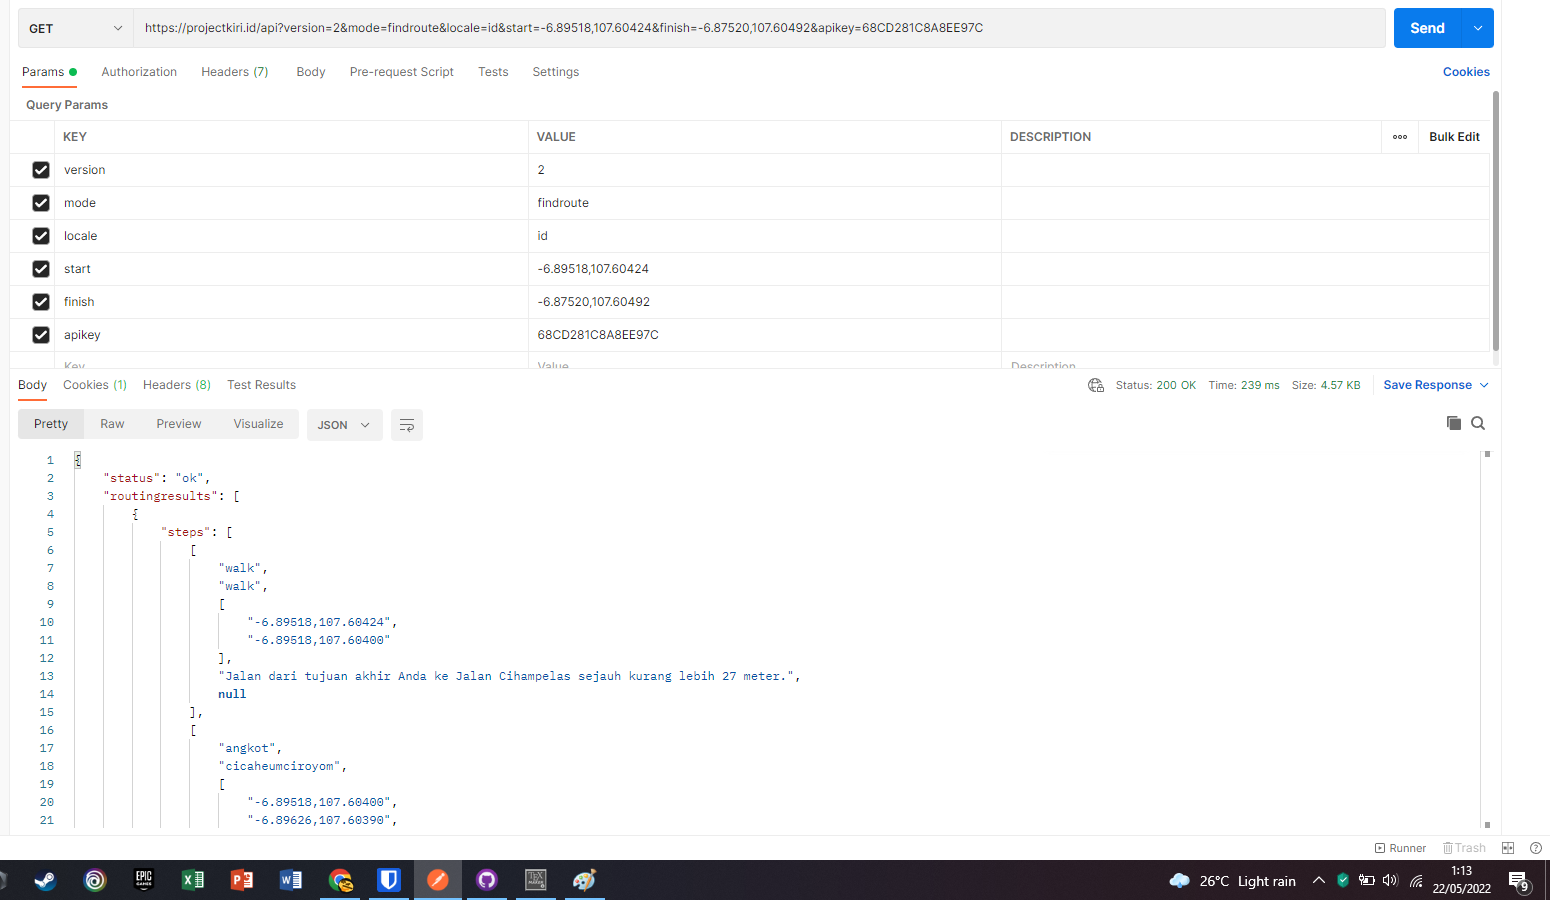
\includegraphics[width=0.74\linewidth]{apikiri-routing}
    \caption[Penggunaan API KIRI untuk layanan pencarian rute]{Penggunaan API KIRI untuk layanan pencarian rute menggunakan Postman. Gambar ini menunjukkan hasil pencarian rute dari Cihampelas Walk ke UNPAR.}
    \label{fig:kiri-api-routing-usage}
\end{figure}

\vspace{\baselineskip}
\textbf{\textit{\large{Smart Direction}}}
\label{sec:kiri-api-smartdir}

Layanan terakhir dari API ini adalah layanan \textit{smart direction}, yang merupakan gabungan dari kedua layanan sebelumnya. Berbeda dengan kedua layanan tadi, yang harus mengakses API secara manual (dengan mengirimkan permintaan GET), layanan ini tidak memerlukan pengguna untuk mengirim permintaan tersebut secara manual\textemdash layanan ini sudah otomatis mengirimkan permintaan tersebut. Berbeda dengan kedua layanan sebelumnya pula, layanan ini tidak memerlukan dibuatnya kunci API terlebih dahulu.

Layanan ini bekerja dengan menyuruh peramban pengguna untuk langsung mengakses halaman web KIRI yang sudah langsung menunjukkan rute yang perlu ditempuh untuk pergi dari lokasi satu ke lokasi lainnya. Untuk melakukan hal ini, layanan ini memerlukan sebuah URL, yang memiliki format sebagai berikut:

\begin{verbatim}
  https://projectkiri.id?start=<lokasi awal>&finish=<lokasi akhir>&locale=<locale>
\end{verbatim}
\noindent
Dapat dilihat bahwa URL tersebut memiliki tiga buah parameter, yaitu:

\begin{itemize}
	\item \verb|start|\\
	\textbf{Kemungkinan nilai:} Nilai \latlon lokasi, atau nama lokasi tersebut\\
	Parameter ini berisi lokasi yang ingin digunakan sebagai lokasi mulainya pencarian rute.
	\item \verb|finish|\\
	\textbf{Kemungkinan nilai:} Nilai \latlon lokasi, atau nama lokasi tersebut\\
	Parameter ini berisi lokasi yang merupakan tujuan akhir yang ingin dicapai dalam pencarian rute.
	\item \verb|locale| (opsional)\\
	\textbf{Kemungkinan nilai:} \verb|id| atau \verb|en|\\
	Menentukan dalam bahasa apa hasil pencarian rutenya akan ditampilkan (bahasa Indonesia atau bahasa Inggris). Jika parameter ini tidak diberikan oleh pengguna, maka bahasa yang akan digunakan adalah bahasa yang terakhir dipakai di halaman web KIRI sendiri.
\end{itemize}
\vspace{\baselineskip}\noindent
Misalkan pengguna ingin mencari rute dari Cihampelas Walk ke Universitas Katolik Parahyangan, dan menampilkan langkah-langkah yang harus ditempuh dalam rutenya dalam bahasa Indonesia. Pengguna dapat memasukkan URL berikut ke peramban mereka.

\begin{verbatim}
            https://projectkiri.id?start=ciwalk&finish=unpar&locale=id
\end{verbatim}
\noindent
Jika URL tersebut sudah dimasukkan ke kotak \textit{link} pada peramban, halaman yang akan ditampilkan akan terlihat seperti pada gambar \ref{fig:kiri-api-smartdirections-usage}.

\begin{figure}[ht]
    \centering
    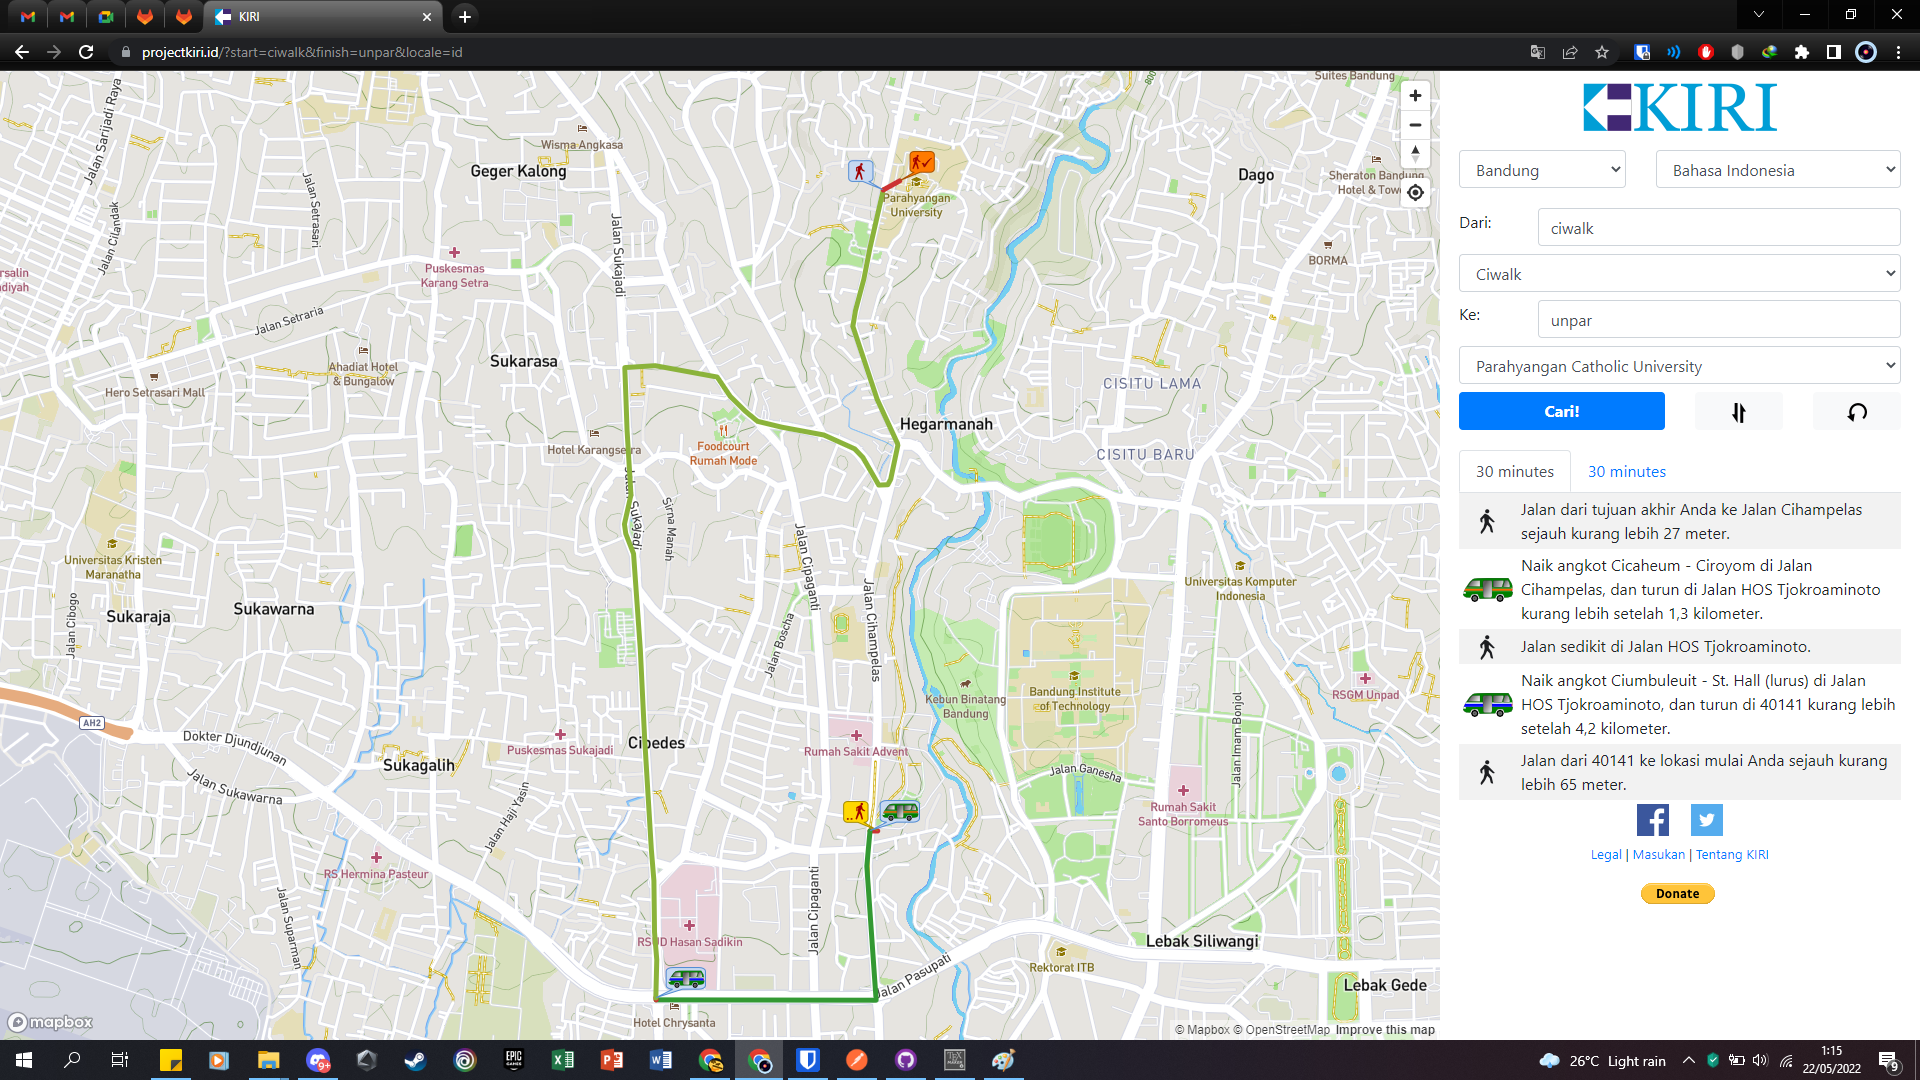
\includegraphics[width=0.74\linewidth]{apikiri-smartdirections}
    \caption[Penggunaan API KIRI untuk layanan \textit{smart direction}]{Penggunaan API KIRI untuk layanan \textit{smart direction}, dari Cihampelas Walk ke UNPAR.}
    \label{fig:kiri-api-smartdirections-usage}
\end{figure}
		
		\item \textbf{Mempelajari perkakas-perkakas \cl sejenis.}\\
		{\bf Status :} Ditambahkan pada Skripsi 1.\\
		{\bf Hasil :} Untuk pembuatan perangkat lunak dalam skripsi ini, ada empat buah perkakas \cl yang akan diamati sebagai aplikasi sejenis. Dua dari empat aplikasi pertama adalah \chromewebstorecli dan \textit{iTunes Search API}. Selain dua perkakas tersebut, ada dua perkakas lainnya yang bisa digunakan sebagai referensi, tetapi tidak dapat dieksplorasi, karena kedua aplikasi tersebut tidak berhasil dijalankan dengan sempurna. Kedua perkakas tersebut adalah \ubercli dan \googlemapscli .

\textbf{\large{\chromewebstorecli}\footnote{\href{https://github.com/pandawing/node-chrome-web-store-item-property-cli}{https://github.com/pandawing/node-chrome-web-store-item-property-cli}}}
\label{sec:similarapps-chromewebstore}

Perkakas \cl ini merupakan ekstensi dari sebuah aplikasi lain yang memiliki fungsi yang \mbox{sama}, yaitu Chrome \textit{Web Store Item Property}.\footnote{\href{https://github.com/pandawing/node-chrome-web-store-item-property}{https://github.com/pandawing/node-chrome-web-store-item-property}} Perangkat lunak \chromewebstorecli ini merupakan perangkat lunak yang akan memanggil fungsi API untuk mendapatkan metadata dari sebuah ekstensi pada \textit{web store} peramban Google Chrome. Perbedaan dari perkakas ini dengan aplikasi dasarnya adalah bahwa perkakas ini dapat digunakan sebagai perkakas \textit{command line}, sedangkan aplikasi dasarnya hanya bisa digunakan dalam perangkat lunak lainnya sebagai pemanggil fungsi API.

\textbf{Penggunaan}
\label{sec:similarapps-chromewebstore-usage}

Perkakas ini dapat digunakan melalui \textit{command prompt} dengan cara mengetikkan perintah sebagai berikut.

\begin{verbatim}
                   chrome-web-store-item-property <identifier>
\end{verbatim}

Dengan \verb|identifier| berupa ID dari ekstensi yang diinginkan. Jadi, misal pengguna \mbox{memasukkan} \verb|gighmmpiobklfepjocnamgkkbiglidom| sebagai ID yang akan digunakan sebagai \textit{identifier}, maka perkakas ini akan mengembalikan \textit{metadata} dari ekstensi ``AdBlock'' sebagai keluarannya. Contoh \mbox{penggunaan} perkakas ini dapat dilihat di gambar \ref{fig:similarapps-chromewebstorecli}.

\begin{figure}[ht]
    \centering
    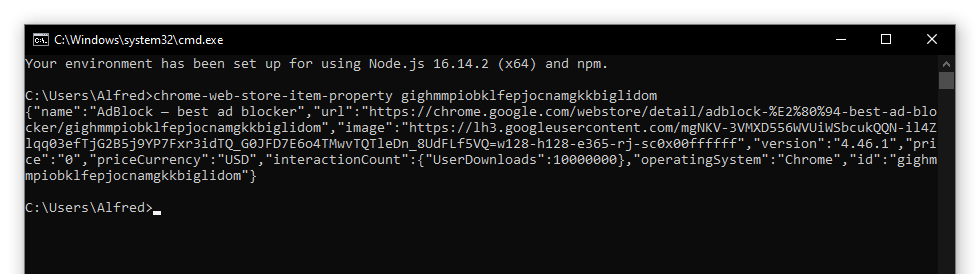
\includegraphics[width=0.75\linewidth]{chromewebstorecli}
    \caption[Contoh penggunaan perkakas \chromewebstorecli]{Contoh penggunaan perkakas \chromewebstorecli.}
    \label{fig:similarapps-chromewebstorecli}
\end{figure}

Sedangkan, keluaran dari perkakas ini merupakan sebuah objek JSON dengan properti-properti sebagai berikut.

\begin{itemize}
	\item \verb|name|\\
	Nama dari ekstensi yang dicari \textit{metadata}-nya.
	\item \verb|url|\\
	URL halaman web dari ekstensi yang dicari di \textit{web store} Google Chrome.
	\item \verb|image|\\
	Logo (dan ikon \textit{thumbnail}) dari ekstensi yang dicari metadatanya.
	\item \verb|version|\\
	Nomor versi dari ekstensi.
	\item \verb|price|\\
	Harga dari ekstensi. Jika ekstensi tidak memiliki harga yang perlu dibayarkan (gratis), properti ini akan bernilai \verb|0|.
	\item \verb|priceCurrency|\\
	Kode mata uang dari harga ekstensi. Jika ekstensi tidak memiliki harga yang perlu dibayarkan, properti ini akan berisi ``\verb|USD|``.
	\item \verb|interactionCount|\\
	Properti ini berisi interaksi-interaksi pengguna yang tercatat sebagai data di halaman \textit{web store} ekstensi. Pada saat pembuatan skripsi ini, properti ini hanya memiliki satu buah subproperti, yaitu \verb|userDownloads|, yang menandakan berapa kali ekstensi ini telah diunduh oleh pengguna di manapun.
	\item \verb|operatingSystems|\\
	Menandakan di peramban mana ekstensi versi ini dapat diinstal. Karena ekstensi-ekstensinya berada di \textit{web store} Chrome,
	\item \verb|ratingValue| (tidak digunakan lagi)\\
	Peringkat yang diberikan oleh para pengguna ekstensi ini. Nilai dari properti ini berupa skala desimal dari 0.00 sampai dengan 5.00. Di versi terbaru dari perkakas ini, properti ini tidak lagi tersedia dalam keluarannya.
	\item \verb|ratingCount| (tidak digunakan lagi)\\
	Jumlah pengguna yang telah menilai/memberi peringkat ke ekstensi ini. Di versi terbaru dari perkakas ini, properti ini tidak lagi tersedia dalam keluarannya.
	\item \verb|id|\\
	Properti ini mengandung ID dari ekstensi tersebut. Nilai dari properti ini akan sama dengan ID yang digunakan sebagai parameter masukan perkakas.
\end{itemize}

\vspace{\baselineskip}
\textbf{\large{\itunesapi}\footnote{\href{https://github.com/awcross/itunes-search-api}{https://github.com/awcross/itunes-search-api}}}
\label{sec:similarapps-itunesapi}

Perkakas \cl ini berfungsi untuk melakukan pencarian melalui API iTunes, sehingga seakan-akan pengguna langsung melakukan pencarian di iTunes sendiri. Hasil pencarian yang dilakukan termasuk judul lagu, nama artis, ataupun nama album, dan pengguna dapat memilih secara spesifik objek apa yang ingin dicari.

\textbf{Penggunaan}
\label{sec:similarapps-itunesapi-usage}

Perkakas ini dapat digunakan melalui \textit{command prompt} dengan cara mengetikkan perintah sebagai berikut.

\begin{verbatim}
                       itunes-search-api <input> [<options>]
\end{verbatim}

Dengan \verb|input| berupa nama dari objek yang dicari. Perkakas ini juga memiliki opsi yang masing-masing memiliki parameter tersendiri untuk mempersempit hasil pencarian. Adapun opsi-opsi tersebut dapat dilihat di daftar di bawah ini.

\begin{itemize}
	\item \verb|country|\\
	\textbf{Kemungkinan nilai:} Kode negara dua huruf\\
	Opsi ini menerima parameter berupa kode negara asal dari album atau artis yang dicari.
	\item \verb|entity|\\
	\textbf{Kemungkinan nilai:} \verb|song|, \verb|musicArtist|, atau \verb|album|\\
	Menandakan jenis objek/entitas yang ingin dicari. Opsi ini dapat bernilai \verb|song| untuk pencarian berbasis judul lagu, \verb|musicArtist| untuk pencarian nama artis, atau \verb|album| untuk pencarian nama album. Jika opsi ini tidak dipakai, objek apapun yang memiliki kemiripan dengan \verb|input| dalam salah satu dari ketiga properti ini akan muncul dalam hasil pencarian.
	\item \verb|limit|\\
	\textbf{Kemungkinan nilai:} Bilangan bulat positif\footnote{Opsi ini juga menerima bilangan bulat negatif, tetapi menggunakan sebuah bilangan bulat negatif akan menghilangkan pengaruh opsi ini terhadap hasil keluaran.}\\
	Jumlah hasil pencarian maksimal yang ingin ditampilkan dalam keluaran.
\end{itemize}

Sedangkan, keluaran dari perkakas ini merupakan sebuah objek JSON yang memiliki dua properti utama, yaitu:

\begin{itemize}
	\item \verb|resultCount|\\
	Properti ini berisi bilangan bulat yang menandakan berapa buah objek yang terdapat dalam hasil pencarian.
	\item \verb|results|\\
	\textit{Array} yang berisi kumpulan objek yang terdapat di dalam hasil pencarian. Objek-objek ini akan dikembalikan berupa sebuah \textit{array} lain yang berisi seluruh properti dari masing-masing objek. Apa saja properti yang diikutkan dalam \textit{array} tersebut tergantung tipe dari objek dalam hasil pencarian.
\end{itemize}

Adapun contoh penggunaan dan hasil keluaran perkakas ini dapat dilihat di gambar \ref{fig:similarapps-itunesapi}.

\begin{figure}[ht]
    \centering
    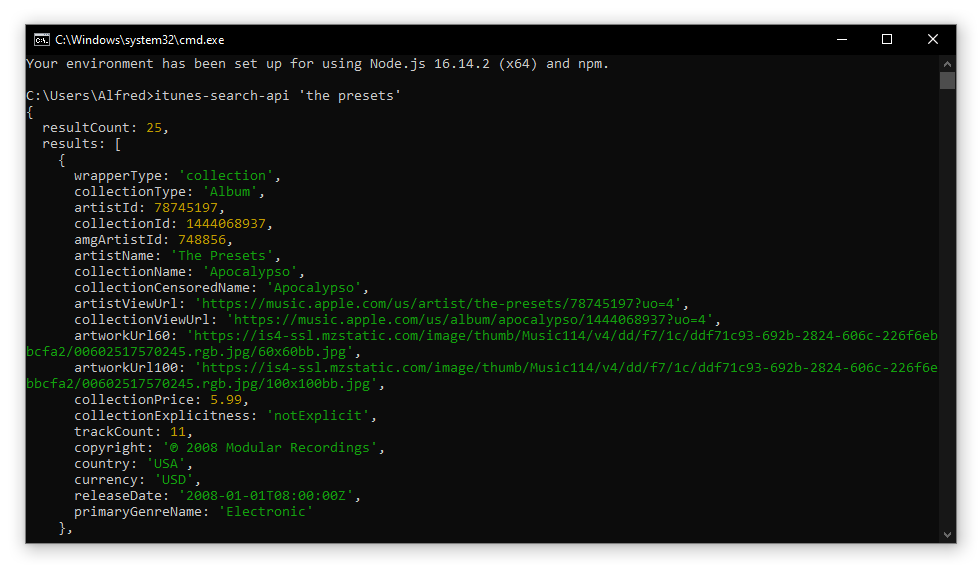
\includegraphics[width=0.75\linewidth]{itunesapi}
    \caption[Contoh penggunaan perkakas \itunesapi]{Contoh penggunaan perkakas \itunesapi. Gambar hanya memuat satu objek untuk menghemat tempat.}
    \label{fig:similarapps-itunesapi}
\end{figure}

\textbf{\large{\ubercli}\footnote{\href{https://github.com/jaebradley/uber-cli}{https://github.com/jaebradley/uber-cli}}}
\label{sec:similarapps-ubercli}

\ubercli merupakan sebuah perkakas \cl yang dapat digunakan untuk dua fungsi utama. Fungsi pertama dari perkakas ini adalah untuk mendapatkan estimasi untuk seberapa lama waktu yang diperlukan untuk servis taksi \textit{online} dari Uber untuk mencapai lokasi yang ingin dituju, sedangkan fungsi keduanya adalah untuk mengestimasi berapa harga yang harus dibayarkan untuk memakai \mbox{servis} tersebut. 
\newline\newline\noindent
Fungsi yang pertama dapat dilakukan memanggil perintah dengan format sebagai berikut.

\begin{verbatim}
                               uber time <alamat>
\end{verbatim}

\verb|uber| merupakan perintah dasar dari perkakas ini. \verb|time| merupakan parameter yang menandakan bahwa pengguna ingin menggunakan servis prediksi waktu dari perkakas ini. Selain itu, pengguna harus memasukkan alamat yang ingin dituju sebagai parameter akhir dari perintah yang akan digunakan sebagai masukan. Jika sintaksnya sudah benar, perintah tersebut akan bisa diproses oleh perkakas dengan cara mengirimkan pesan hasil konversi perintah tersebut ke API Uber. Setelah pemrosesan pesan tersebut berhasil, perkakas ini akan menampilkan sebuah keluaran dengan format yang dapat dilihat di gambar \ref{fig:similarapps-ubercli-time}. Perlu diperhatikan juga bahwa keluaran yang dihasilkan oleh perkakas ini akan meliputi seluruh jenis servis yang disediakan oleh Uber.

\begin{figure}[ht]
    \centering
    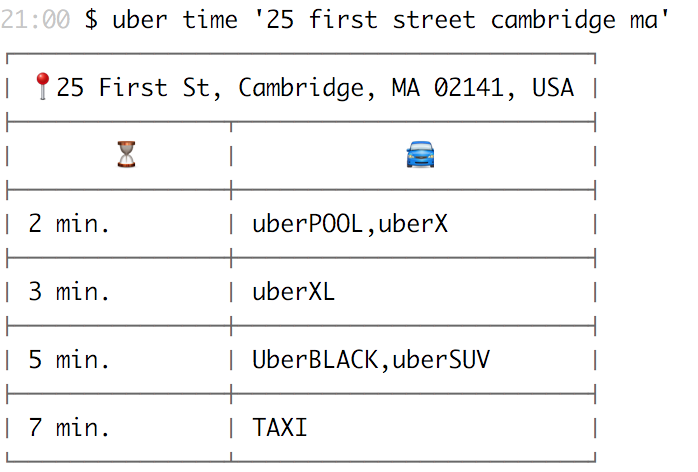
\includegraphics[width=0.425\linewidth]{ubercli-time}
    \caption[Contoh penggunaan perkakas \ubercli (\textit{time})]{Contoh penggunaan fitur prediksi waktu perjalanan untuk perkakas \ubercli.\protect\footnotemark}
    \label{fig:similarapps-ubercli-time}
\end{figure}
\footnotetext{\href{https://github.com/jaebradley/uber-cli}{https://github.com/jaebradley/uber-cli}}

Sedangkan, untuk memanggil fungsi kedua dari perkakas ini, pengguna dapat dilakukan dengan \linebreak memanggil perintah dengan format berikut.

\begin{verbatim}
                  uber price -s <alamat awal> -e <alamat akhir>
\end{verbatim}

Untuk sintaks ini, \verb|uber| memiliki fungsi yang sama dengan sintaks untuk fungsi pertama dari perkakas. \verb|price| merupakan penanda untuk perkakas bahwa pengguna ingin menggunakan servis untuk \linebreak mengetahui perkiraan harga layanan Uber. Selanjutnya, perkakas akan meminta dua buah opsi beserta parameternya masing-masing. Pertama, opsi \verb|-s|, berarti \textit{start}, yang akan meminta sebuah parameter berupa lokasi yang ingin dipakai sebagai lokasi awal perkiraan harga layanan Uber. Sedangkan opsi \verb|-e|, berarti \textit{end}, akan meminta sebuah parameter berupa lokasi yang ingin dipakai sebagai lokasi akhir jasa perkiraan harga.
\newline\newline\noindent
Adapun keluaran dari fungsi kedua ini dapat dilihat di gambar \ref{fig:similarapps-ubercli-price}. Sama seperti keluaran untuk fungsi pertamanya, keluaran untuk fungsi kedua perkakas ini juga meliputi seluruh jasa yang disediakan oleh Uber.

\begin{figure}[ht]
    \centering
    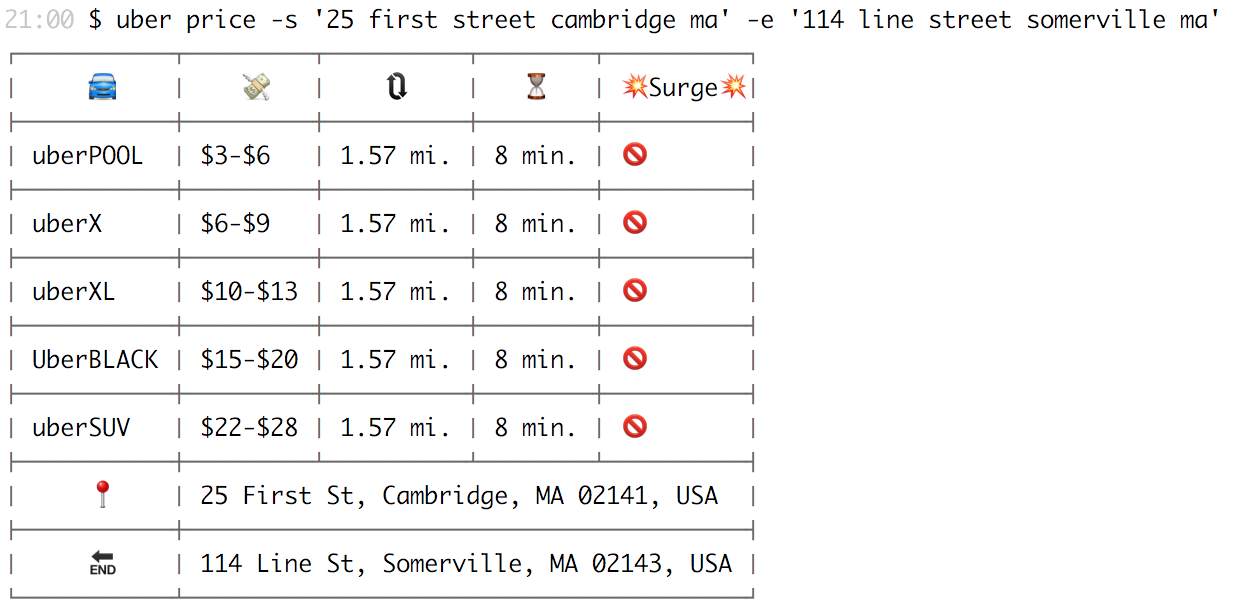
\includegraphics[width=0.75\linewidth]{ubercli-price}
    \caption[Contoh penggunaan perkakas \ubercli (\textit{price})]{Contoh penggunaan fitur prediksi harga perjalanan untuk perkakas \ubercli.\protect\footnotemark}
    \label{fig:similarapps-ubercli-price}
\end{figure}
\footnotetext{Gambar diambil dari \href{https://github.com/jaebradley/uber-cli}{https://github.com/jaebradley/uber-cli}}

\textbf{Permasalahan}
\label{sec:similarapps-ubercli-problem}

Seperti telah dijelaskan di awal bab ini, perkakas ini tidak dapat digunakan. Kesimpulan yang diambil oleh penulis mengenai alasan perkakas ini tidak dapat dijalankan adalah dikarenakan oleh penggunaan API dan modul-modul yang telah usang (\textit{deprecated}). Kesimpulan ini diambil oleh penulis karena dua alasan utama. Pertama, pada awalnya, perkakas ini tidak dapat dijalankan karena API Google \textit{Maps} yang dipakai mengandung baris kode berikut didalamnya.

\begin{verbatim}
           exports.placesAutoCompleteSessionToken = require('uuid/v4');
\end{verbatim}
\vfill\newpage % prevent widow
Kode ini merupakan kode yang dipakai untuk mengambil \textit{subpath} dari paket \verb|uuid|, tetapi penggunaannya sudah berubah untuk versi yang lebih barunya. Akan tetapi, setelah diganti baris tersebut ke penggunaan versi barunya pun, perkakas ini masih tetap tidak dapat dijalankan\textemdash sekarang perkakas ini justru mengembalikan sebuah error. Singkatnya, error tersebut menunjukkan bahwa perkakas \mbox{mencoba} untuk mengakses API Uber dengan menggunakan kredensial OAuth 2.0 yang hanya berlaku untuk versi sebelumnya dari API tersebut. Permasalahan ini merupakan permasalahan yang juga ditemukan oleh beberapa pengguna lain, seperti tertera di halaman \textit{GitHub Issues} dari repositori ini.\footnote{\href{https://github.com/jaebradley/uber-cli/issues/87}{https://github.com/jaebradley/uber-cli/issues/87}} Oleh karena hal ini tidak lagi merupakan masalah kode perangkat lunak, maka perkakas ini dianggap tidak dapat dipakai.

\vspace{\baselineskip}
\textbf{\large{\googlemapscli}\footnote{\href{https://github.com/yujinlim/google-maps-direction-cli}{https://github.com/yujinlim/google-maps-direction-cli}}}
\label{sec:similarapps-googlemapscli}

\googlemapscli merupakan sebuah perkakas \cl yang memiliki kegunaan yang mirip dengan KIRI, hanya saja perkakas ini tidak secara spesifik mengharuskan penggunaan angkot, atau transportasi umum lainnya. Singkatnya, perkakas ini memiliki fungsi seperti sebuah GPS. Untuk menggunakannya, pengguna harus memasukkan perintah dengan bentuk sebagai berikut.

\begin{verbatim}
                      direction <lokasi awal> <lokasi akhir>
\end{verbatim}

Setelah pengguna memasukkan perintah tersebut dengan benar, perkakas ini akan mengirim permintaan ke API Google \textit{Maps}, di mana jika prosesnya berhasil, keluarannya akan berupa langkah-langkah yang harus ditempuh untuk sampai ke lokasi akhir, beserta di jarak berapa langkah tersebut harus diambil, relatif terhadap langkah sebelumnya. Adapun penggunaan dari perkakas ini dapat dilihat di gambar \ref{fig:similarapps-googlemapscli}.

\begin{figure}[ht]
    \centering
    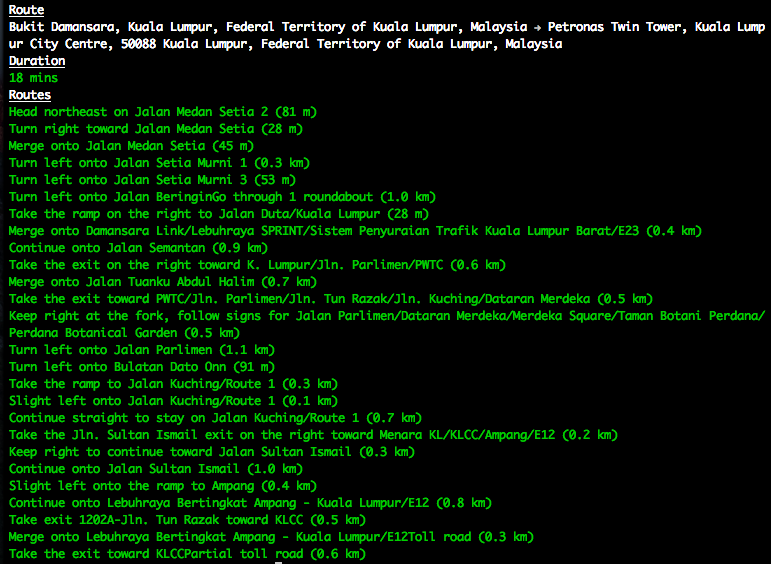
\includegraphics[width=0.66667\linewidth]{googlemapscli}
    \caption[Contoh penggunaan perkakas \googlemapscli]{Contoh penggunaan perkakas \googlemapscli.\protect\footnotemark}
    \label{fig:similarapps-googlemapscli}
\end{figure}
\footnotetext{Gambar diambil dari \href{https://github.com/yujinlim/google-maps-direction-cli}{https://github.com/yujinlim/google-maps-direction-cli}}

\textbf{Permasalahan}
\label{sec:similarapps-googlemapscli-problem}

Seperti tertulis di awal bab ini, perkakas ini juga tidak bisa digunakan. Alasan perkakas ini tidak dapat digunakan lagi-lagi merupakan masalah teknikal, yaitu diperbaruinya API Google \textit{Maps}. Lebih spesifiknya, semenjak 2018, \textit{Google} tidak lagi memperbolehkan penggunaan API Google \textit{Maps} tanpa kunci API, yang sayangnya tidak hanya mendasari perkakas ini, tetapi juga kunci API ini tidak bisa didapatkan tanpa membayarkan biaya tertentu. Oleh karena itu, perkakas ini dianggap tidak bisa lagi dijalankan.
		
		\item \textbf{Mempelajari bahasa pemrograman C serta mempelajari dokumentasi-dokumentasi dari seluruh modul yang dibutuhkan untuk pembuatan perangkat lunak.}\\
		{\bf Status :} Ada sejak rencana kerja skripsi.\\
		{\bf Hasil :} Fungsi bawaan dari bahasa C yang akan digunakan dalam pembuatan perangkat lunak dalam skripsi ini adalah fungsi \verb|getopt|.

\vspace{\baselineskip}
\textbf{\large{getopt} \cite{loosemore:2022:gnuclibrary}}
\label{sec:cmodules-getopt}

\verb|getopt| merupakan sebuah fungsi yang dapat mengautomasi pekerjaan-pekerjaan yang berhubungan dengan penerimaan opsi-opsi untuk \cl berbasis UNIX.
\newline\newline\noindent
Fungsi \verb|getopt| dapat dipanggil dengan format sebagai berikut.

\begin{verbatim}
                           getopt (argc, argv, <options>)
\end{verbatim}

Seluruh kode ini dapat dimasukkan ke suatu variabel berupa sebuah karakter yang merepresentasikan opsi yang ingin digunakan. \verb|argc| merupakan jumlah argumen yang terdapat dalam masukan, \linebreak sedangkan argv merupakan sebuah \textit{array} yang berisi argumen-argumen tersebut.
\newline\newline
Selain itu, penggunaan \verb|getopt| juga akan memakai variabel-variabel tertentu, yang nilainya akan diisi oleh fungsi \verb|getopt| tersebut sendiri. Variabel-variabel ini beserta penjelasannya dapat dilihat di daftar berikut.\footnote{\href{https://www.gnu.org/software/libc/manual/html\_node/Using-Getopt.html}{https://www.gnu.org/software/libc/manual/html\_node/Using-Getopt.html}}
\begin{itemize}
	\item \verb|opterr|\\
	Isi dari variabel ini akan memberi sinyal ke perangkat lunak/perkakas yang menentukan apakah \verb|getopt| akan mengirim pesan ke \textit{error stream} atau tidak. Jika variabel ini bukan bernilai 0, maka pesan \textit{error} akan dikirim. Sebaliknya, jika variabel ini bernilai 0, \verb|getopt| tidak akan mengirim pesan \textit{error} apapun, tetapi tetap akan mengembalikan sebuah karakter tanda tanya (\verb|?|) sebagai tanda bahwa sebuah \textit{error} telah terjadi.
	\item \verb|optopt|\\
	Ketika \verb|getopt| menemukan sebuah karakter yang tidak didefinisikan dalam kumpulan opsi, atau sebuah opsi yang tidak disertai argumen yang diperlukan, karakter tersebut akan disimpan di variabel ini.
	\item \verb|optind|\\
	Variabel ini digunakan oleh \verb|getopt| sebagai indeks untuk \textit{array} \verb|argv|. Jika seluruh argumen sudah diproses, nilai variabel ini dapat digunakan untuk menentukan argumen mana yang merupakan argumen tambahan yang tidak terpakai. Nilai dari variabel ini dimulai dari 1.
	\item \verb|optarg|\\
	Jika opsi yang sedang diproses memerlukan argumen, variabel ini adalah tempat dimana argumen tersebut akan disimpan.
	\item \verb|<options>|\\
	Variabel ini merupakan salah satu variabel yang tertera di format pemanggilan \verb|getopt| di atas. Variabel ini berupa \textit{string} yang menandakan karakter-karakter apa saja yang menjadi opsi yang mungkin dalam perkakas tersebut, beserta tipenya. Jika karakter opsi:
	
	\begin{itemize}
		\item Diikuti dengan titik dua (\verb|:|), maka opsi tersebut memiliki argumen yang bersifat wajib.
		\item Diikuti dengan titik dua ganda (\verb|::|), maka opsi tersebut memiliki argumen yang bersifat opsional.
		\item Tidak diikuti apa-apa, maka opsi tersebut merupakan opsi tidak berarguman.
	\end{itemize}
	
\end{itemize}
\noindent
Untuk memberikan gambaran yang lebih baik mengenai penggunaan fungsi \verb|getopt|, berikut merupakan contoh perangkat lunak berbasis \cl sederhana yang menggunakan fungsi tersebut. Perangkat lunak ini akan menerima masukan berupa opsi tidak berparameter \verb|-a| dan/atau opsi berparameter \verb|-b|. Untuk opsi \verb|-a|, perangkat lunak ini akan mengeluarkan nilai 0 jika opsi \verb|-a| tidak dipakai, dan 1 jika opsi tersebut dipakai. Sebagai keluaran keduanya, perangkat lunak ini akan mengeluarkan isi parameter dari opsi \verb|-b|, atau \verb|NULL| jika opsi \verb|-b| tidak dipakai.

\begin{lstlisting}[language=C, caption=Contoh sederhana penggunaan getopt, label=code:getopt-usage]
#include <ctype.h>
#include <stdio.h>
#include <stdlib.h>
#include <unistd.h>

int main(int argc, char **argv) {
    int aflag = 0;
    char *bvalue = NULL;
    int index;
    int args;

    opterr = 0;

    while ((args = getopt(argc, argv, ":ab:")) != -1)
        switch (args) {
	        case 'a':
	            aflag = 1;
	            break;
	        case 'b':
	            bvalue = optarg;
	            break;
	        case ':':
    	        if (optopt == 'b') {
	                fprintf(stderr, "Option -%c requires an argument.\n", optopt);
	            }
	            return 1;
	        case '?':
	            if (isprint(optopt)) {
	                fprintf(stderr, "Unknown option `-%c'.\n", optopt);
	            }
	            else fprintf(stderr, "Unknown option character `\\x%x'.\n", optopt);
	            return 1;
	        default:
	            abort();
        }

    printf("aflag = %d, bvalue = %s\n", aflag, bvalue);
    for (index = optind; index < argc; index++)
        printf("Non-option argument %s\n", argv[index]);

    return 0;
}
\end{lstlisting}

\textbf{getopt-long}
\label{sec:cmodules-getopt-long}

Ada pula versi \verb|getopt| yang memungkinkan perangkat lunak untuk menerima dua jenis opsi\textemdash opsi versi pendek berupa sebuah karakter singular, seperti pada \verb|getopt| biasa, dan/atau opsi panjang bergaya GNU, berupa sebuah kata.

\verb|getopt-long| juga memiliki seluruh variabel-variabel yang dimiliki oleh \verb|getopt|, hanya saja \linebreak \verb|getopt-long| memiliki sebuah variabel tambahan berupa struktur, yaitu \verb|long_options|. Variabel ini merupakan sebuah struktur berupa \textit{array} yang berisi beberapa \textit{array} lainnya, di mana \textit{array-array} lain in merupakan masing-masing opsi dari fungsi \verb|getopt-long| tersebut. Tiap-tiap \textit{array} tersebut memiliki variabel-variabel berikut:

\begin{itemize}
	\item \verb|name|\\
	Variabel ini merupakan nama panjang dari opsi.
	\item \verb|has_arg|\\
	Variabel ini merupakan penanda apakah opsi memerlukan argumen atau tidak. Nilai yang \linebreak mungkin dalam variabel ini adalah \verb|no_argument|, \verb|required_argument|, atau \verb|optional_argument|.
	\item \verb|flag| \& \verb|val|\\ 
	Kedua variabel ini menandakan bagaimana sebuah opsi akan diberlakukan ketika diterima oleh \verb|getopt-long|. Variabel \verb|flag| dapat diisi dengan penunjuk (\textit{pointer}) ke suatu variabel lain yang akan diisi dengan isi dari variabel \verb|val| untuk menandakan bahwa \verb|getopt-long| telah berhasil memproses opsi tersebut. Di lain sisi, jika variabel ini berisi \textit{null pointer}, maka fungsi \verb|getopt-long| akan mengembalikan isi dari variabel \verb|val|.
\end{itemize}
\noindent
Struktur ini harus diakhiri dengan sebuah \textit{array} tambahan yang seluruh variabelnya bernilai 0.
\newline\newline
Untuk menjelaskan lebih lanjut mengenai cara penggunaan \verb|getopt-long|, berikut merupakan \linebreak contoh perangkat lunak berbasis \cl sederhana yang menggunakan fungsi tersebut. Adapun perangkat lunak ini memiliki spesifikasi sebagai berikut:

\begin{itemize}
	\item Perangkat lunak ini akan menerima masukan dari penggunaan opsi-opsi serta parameternya.
	\item Keluaran dari perangkat lunak ini adalah opsi apa saja yang dipilih, serta parameter yang \linebreak diberikan (jika ada).
	\item Opsi pertama yang disediakan adalah \verb|-a| atau \verb|--args| yang merupakan opsi tidak berargumen.
	\item Opsi kedua yang disediakan adalah \verb|-n| atau \verb|--noargs|, yang merupakan opsi yang membutuhkan sebuah argumen.
	\item Opsi ketiga dan keempat merupakan penanda mode keluaran, yaitu \verb|--short| dan \verb|--long|. Jika opsi \verb|--long| digunakan, maka perangkat lunak ini akan mengeluarkan versi panjang dari keluaran, sedangkan jika opsi \verb|--short| digunakan, maka perangkat akan mengeluarkan versi pendek dari keluaran.
\end{itemize}

\begin{lstlisting}[language=C, caption=Contoh sederhana penggunaan getopt-long, label=code:getopt-usage-long]
#include <stdio.h>
#include <stdlib.h>
#include <getopt.h>

int main(int argc, char **argv) {
    int option;
    static int verbose;

    while (1) {
        static struct option long_options[] = {
                {"long", 0, &verbose, 1},
                {"short", 0, &verbose, 0},
                {"noargs", 0, 0, 'n'},
                {"args", 1, 0, 'a'},
                {0, 0, 0, 0}};
        int option_index = 0;
        option = getopt_long(argc, argv, "na:", long_options, &option_index);

        if (option == -1)
            break;
        switch (option) {
	        case 0:
    	        if (verbose) {
	                printf("Print mode is set to: %s", long_options[option_index].name);
	            }
	            else
	                printf("Print mode is set to: %s", long_options[option_index].name);
	            putchar('\n');
	            break;

    	    case 'n':
	            if (verbose == 1) {
	                printf("Option '%s' was picked. This option does not require any arguments.", long_options[option_index].name);
    	        }
	            else
	                printf("Argumentless option '%s' was picked.", long_options[option_index].name);
	            putchar('\n');
	            break;

    	    case 'a':
	            if (verbose == 1) {
	                printf("Option '%s' was picked with argument '%s'.", long_options[option_index].name, optarg);
	            }
	            else
	                printf("a = %s", optarg);
	            putchar('\n');
	            break;

    	    case '?':
	            break;
	
	        default:
	            abort();
        }
    }

    if (optind < argc)
    {
        printf("Arguments passed without a corresponding option (argv): ");
        while (optind < argc) {
            printf("%s ", argv[optind++]);
        }
        putchar('\n');
    }

    exit(0);
}
\end{lstlisting}

		\item \textbf{Melakukan analisis dan desain perangkat lunak yang akan dibangun.}\\
		{\bf Status :} Ada sejak rencana kerja skripsi\textemdash desain akan dilakukan di Skripsi 2.\\
		{\bf Hasil :} Pada skripsi ini, akan dibangun sebuah aplikasi berupa perkakas \cl yang merupakan ekstensi dari sebuah aplikasi berbasis web lain, yaitu KIRI. Perkakas ini akan menjadi ekstensi KIRI dengan cara memungkinkan penggunanya untuk mengakses fungsi-fungsi API KIRI dari \cl milik perangkat mereka masing-masing. Fungsi utama dari perkakas ini tentunya sama dengan KIRI sendiri, yaitu membantu navigasi dari satu lokasi ke lokasi lain dengan menggunakan angkot.

Walaupun begitu, aplikasi ini akan memiliki dua fungsi utama yang berhubungan satu sama lain, yaitu pencarian lokasi, dan penunjukkan rute dengan angkot.

\begin{itemize}
	\item Pencarian lokasi\\
	Pencarian lokasi merupakan fungsi utama pertama dari perkakas ini. Untuk fungsi ini, masukan langsung dari pengguna yang akan diterima oleh perkakas adalah kata kunci dari sebuah lokasi yang ingin dicari. Kemudian, perkakas akan memprosesnya melalui API KIRI, lalu \linebreak mengembalikan nama lokasi tersebut, serta nilai \textit{latitude} dan \textit{longitude}-nya, sebagai keluaran akhir dari proses tersebut.
	\item Pencarian rute\\
	Pencarian rute dengan angkot merupakan fungsi utama kedua, sekaligus fungsi umum dari \linebreak perkakas ini. Dalam fungsi ini, perkakas akan meminta masukan langsung pengguna berupa nilai \latlon dari lokasi awal serta lokasi akhir dari perjalanan pengguna. Setelah masukan ini berhasil diterima dan diproses, perkakas akan mengeluarkan keluaran akhir berupa langkah-langkah yang harus diambil oleh pengguna untuk pergi dari lokasi awal ke lokasi akhir, dengan memanfaatkan jasa angkot yang ada.
\end{itemize}
\noindent
Berikut merupakan opsi-opsi yang akan disediakan dalam perkakas yang akan dibangun.

\begin{itemize}
	\item \verb|-h|\\
	Perlu diingat juga bahwa aplikasi ini merupakan aplikasi \cl murni, yang berarti bahwa seluruh operasi dari aplikasi ini akan dilakukan tanpa bantuan gambar grafis apapun. Untuk membantu penggunanya dalam mengetahui bagaimana cara menggunakan perkakas ini, tentunya perintah untuk menunjukkan apa perintah-perintah dan opsi-opsi yang tersedia merupakan sebuah keharusan. Hal ini merupakan fungsi satu-satunya dari perintah \verb|--help| ini.
	
	\item \verb|-m <mode>|\\
	Opsi ini merupakan opsi berparameter yang menentukan fitur mana yang ingin digunakan oleh pengguna. Adapun isi dari parameter \verb|mode| yang dapat digunakan adalah sebagai berikut:
	
	\begin{itemize}	
		\item \verb|search|\\
		Parameter ini akan menandakan bahwa pengguna ingin menggunakan fitur \textit{search place} dari perkakas. Untuk mode ini, perkakas akan menerima input dari pengguna dalam bentuk parameter-parameter dari opsi-opsi tambahan. Adapun opsi-opsi tersebut adalah sebagai berikut.
			
		\begin{itemize}
			\item \verb|-r <region>|\\
			Opsi ini merupakan opsi yang akan menerima parameter berupa kode area dari lokasi yang ingin dicari.
			\item \verb|-q <kata kunci>|\\
			Opsi ini merupakan opsi yang akan menerima sebuah \textit{string} sebagai parameternya. \textit{String} ini akan digunakan oleh perkakas sebagai kata kunci untuk pencarian lokasi yang ingin ditemukan oleh pengguna.
		\end{itemize}
	
		\item \verb|route|\\
		Parameter ini akan menandakan bahwa pengguna ingin menggunakan fitur \textit{find route} dari perkakas. Sama seperti mode \verb|--search|, perkakas akan menerima input dari pengguna dari parameter-parameter milik opsi-opsi tambahan. Adapun opsi-opsi tersebut adalah sebagai berikut.
		
		\begin{itemize}
			\item \verb|-s <lokasi awal>|\\
			Opsi ini merupakan opsi yang akan menerima parameter berupa lokasi awal perjalanan pengguna nantinya. Perlu diingat bahwa opsi ini hanya menerima masukan lokasi berupa nilai \latlon dari lokasi tersebut.
			\item \verb|-f <lokasi akhir>|\\
			Opsi ini merupakan opsi yang akan menerima parameter berupa lokasi akhir perjalanan pengguna nantinya. Sama seperti opsi sebelumnya, parameter ini juga hanya menerima masukan lokasi berupa nilai \textit{latitude} dan \textit{longitude}.
			\item \verb|-l <kode bahasa>|\\
			Opsi ini akan menerima parameter yang mengatur bahasa yang akan digunakan oleh perkakas di keluarannya nanti.
		\end{itemize}
		
		\item \verb|routedirect|\\
		Parameter ini merupakan tambahan fitur spesifik untuk perkakas ini, yang merupakan \linebreak gabungan dari fitur pencarian lokasi dan pencarian rute. Fitur ini akan menggabungkan kedua fitur tersebut dengan langkah-langkah berikut.
		
		\begin{enumerate}
			\item Perkakas akan menerima lokasi awal dan akhir berupa kata kunci dari pengguna yang dimasukkan kedalam parameter dari opsi masing-masing.
			\item Hasil pencarian kedua lokasi akan dikonfirmasikan terlebih dahulu, apakah lokasi yang \linebreak ditemukan benar merupakan lokasi yang ingin digunakan oleh pengguna atau bukan.
			\item Jika hasil tersebut benar, maka koordinat \latlon dari kedua lokasi tersebut akan disimpan.
			\item Koordinat \latlon dari kedua lokasi tersebut kemudian akan digunakan sebagai masukan untuk langkah kedua dari fitur ini, yaitu pencarian rute.
			\item Hasil dari pencarian rute akan ditampilkan sebagai keluaran akhir dari fitur ini.
		\end{enumerate}
		\noindent
		Adapun parameter yang diperlukan untuk fitur ini merupakan gabungan dari opsi-opsi kedua fitur sebelumnya, yaitu:
		
		\begin{itemize}
			\item \verb|-I <region tempat lokasi awal berada>|\\
			Opsi ini akan menerima parameter berupa kode area lokasi awal yang akan digunakan.
			\item \verb|-E <region tempat lokasi akhir berada>|\\
			Opsi ini akan menerima parameter berupa kode area lokasi akhir yang akan digunakan.
			\item \verb|-S <kata kunci untuk lokasi awal>|\\
			Opsi ini akan menerima parameter berupa kata kunci untuk pencarian lokasi awal yang akan digunakan.
			\item \verb|-F <kata kunci untuk lokasi akhir>|\\
			Opsi ini akan menerima parameter berupa kata kunci untuk pencarian lokasi akhir yang akan digunakan.
			\item \verb|-l <kode bahasa>|\\
			Opsi ini akan menerima parameter yang mengatur bahasa yang akan digunakan oleh perkakas di keluarannya nanti. Opsi ini merupakan opsi yang sama dengan opsi yang digunakan dalam mode \verb|route|.
		\end{itemize}
		
	\end{itemize}
	
\end{itemize}
		
		\item \textbf{Melakukan analisis kebutuhan fitur-fitur perangkat lunak.}		
		\label{sec:num5} \newline
		{\bf Status :} Dipisah dua menjadi nomor ini dan \hyperref[sec:num6]{nomor 6} di Skripsi 1\textemdash tidak dikerjakan.\\
		{\bf Hasil :} Perangkat lunak hasil skripsi ini merupakan ekstensi dari perangkat lunak lainnya, yaitu KIRI. Oleh karena itu, fitur-fitur yang dimiliki oleh perangkat lunak ini akan sama seperti fitur-fitur yang disediakan oleh KIRI.
		
		
		\item \textbf{Melakukan eksplorasi \textit{library} yang dapat digunakan dan memenuhi spesifikasi dalam pembuatan perangkat lunak.}
		\label{sec:num6} \newline
		{\bf Status :} Dipisah dua menjadi nomor ini dan \hyperref[sec:num5]{nomor 5} di Skripsi 1.\\
		{\bf Hasil :} Adapun \textit{library-library} yang dapat digunakan berdasarkan spesifikasi perangkat lunak adalah sebagai berikut.

\textbf{\large{libcurl} \cite{stenberg:2022:everythingcurl}}
\label{sec:cmodules-libcurl}

libcurl merupakan sebuah \textit{library} yang berisi fungsi-fungsi yang disediakan dalam bentuk API bahasa C, untuk digunakan oleh aplikasi-aplikasi bahasa C. Libcurl didesain dengan berorientasi transfer (biasanya transfer berkas), tanpa memerlukan para penggunanya untuk mengerti protokol-protokol yang digunakan dalam proses pentransferan tersebut. Fitur transfer ini dapat dibuat sesederhana mungkin, dan seluruh aturan dan opsi seputar pemindahan berkas tersebut dapat diatur nantinya secara manual melalui opsi-opsi yang ada.

Untuk mulai melakukan transfer berkas, diperlukan juga sebuah \textit{handle} yang perlu diinisialisasikan terlebih dahulu. Adapun cURL memiliki dua jenis \textit{handle}, yaitu \textit{easy handle} dan \textit{multi handle}. 

\vspace{\baselineskip}
\textbf{\textit{Easy Handle}}
\label{sec:cmodules-libcurl-handleeasy}

\textit{Easy handle} dari cURL dapat diinisialisasikan dengan memanggil fungsi \verb|curl_easy_init()|. Setelah itu, untuk mengatur opsi-opsi yang perlu diatur sesuai kebutuhan pengguna, seperti URL yang dituju, \linebreak protokol yang ingin dipakai, koneksi ke port spesifik, dan sebagainya,\footnote{\href{https://curl.se/libcurl/c/curl\_easy\_setopt.html}{https://curl.se/libcurl/c/curl\_easy\_setopt.html}} pengguna harus mengaturnya dengan fungsi \verb|curl_easy_setopt()|. \textit{Handle} ini berhasil diatur opsinya apabila fungsi \verb|curl_easy_| \linebreak \verb|setopt()| tadi mengembalikan \verb|CURLE_OK|. Terakhir, untuk menjalankan transfernya, fungsi yang perlu dipanggil adalah \verb|curl_easy_perform(<easy handle>)|, dengan variabel \verb|<easy handle>| diisi dengan nama dari \textit{easy handle} yang ingin dimulai transfernya.

\textit{Handle} yang telah diatur ini dapat digunakan berulang kali dengan konfigurasi yang sama, sampai entah pengguna mengganti konfigurasi opsi-opsinya kembali, atau \textit{handle}-nya diatur ulang dengan pemanggilan fungsi \verb|curl_easy_reset()|.

\vspace{\baselineskip}
\textbf{\textit{Multi Handle}}
\label{sec:cmodules-libcurl-handlemulti}

\textit{Multi handle} merupakan sebuah \textit{handle} yang dapat memfasilitasi beberapa transfer yang \mbox{dilakukan} secara paralel. Metode pentransferan filenya masih sama dengan \textit{easy handle}, hanya saja untuk \textit{multi handle}, diperlukan sebuah \textit{handle} tambahan yang dapat menampung seluruh \textit{easy handle} yang akan digunakan. Adapun \textit{handle} tipe ini dapat diinisialisasikan dengan memanggil fungsi \verb|curl_multi_init()|, dan untuk mengatur opsi-opsi seputar \textit{multi handle} tersebut, pengguna dapat memanggil fungsi \verb|curl_| \linebreak \verb|multi_setopt()|.

Untuk memulai transfer paralel, tentunya perlu diinisialisasikan dulu masing-masing \textit{easy handle}-nya. Setelah \textit{handle-handle} tersebut diinisialisasikan, \textit{handle} tersebut dapat dimasukkan ke dalam sebuah \textit{multi handle} dengan memanggil fungsi berikut.

\begin{verbatim}
                curl_multi_add_handle(<multi handle>, <easy handle>);
\end{verbatim}
\noindent
Dengan \verb|<easy handle>| merupakan nama dari \textit{easy handle} yang ingin dimasukkan ke dalam \textit{multi handle} tertentu dan \verb|<multi handle>| merupakan nama dari \textit{multi handle}-nya sendiri. Sedangkan, untuk menghapus sebuah \textit{easy handle} dari dari dalam \textit{multi handle}, dapat dipanggil fungsi berikut.

\begin{verbatim}
              curl_multi_remove_handle(<multi handle>, <easy handle>);
\end{verbatim}

Setelah seluruh \textit{easy handle} yang ingin dijalankan dimasukkan ke dalam \textit{multi handle}, \textit{multi handle} tersebut dapat dijalankan dengan menggunakan sebuah \textit{loop} transfer. Adapun isi dari loop ini meliputi tiga langkah utama, yaitu:

\begin{enumerate}
	\item Inisialisasi variabel \verb|transfers_running|\\
	\verb|transfers_running| merupakan sebuah variabel \textit{integer} yang menjadi penanda bagi pengguna mengenai berapa banyak \textit{handle} yang sedang melakukan proses transfer di suatu waktu. Selama nilai variabel ini bukan 0, artinya ada \textit{easy handle} yang belum selesai melakukan proses transfer berkas.
	\item Menjalankan transfer dalam \textit{multi handle}\\
	Langkah selanjutnya adalah menjalankan transfer dalam \textit{mutli handle}, dengan memanggil fungsi \verb|curl_multi_perform|. Adapun fungsi tersebut harus dipanggil dengan format berikut, yaitu:

\begin{verbatim}
           curl_multi_perform(<multi handle>, <transfers_running>)
\end{verbatim}

	\item Menunggu transfer untuk selesai sebelum data diekstraksi\\
	Tentunya sebelum data hasil transfer dapat diekstraksi untuk dipakai, proses transfernya \linebreak sendiri harus selesai terlebih dahulu\textemdash untuk kasus dalam \textit{multi handle} libcurl, seluruh \textit{handle} di dalam \textit{multi handle} harus selesai melakukan transfer terlebih dahulu, atau sampai terjadi \textit{timeout}. Adapun langkah ini dapat diselesaikan entah dengan menggunakan \verb|curl_multi_wait()| atau \verb|curl_multi_poll()|, atau dengan cara manual, yaitu dengan memasukkan deskriptor-deskriptor file serta nilai \textit{timeout} secara manual, dan kemudian menggunakan \verb|select()|, walaupun metode ini tidak dianjurkan karena keterbatasan jumlah deskriptor yang dapat digunakan.\footnote{\href{https://curl.se/libcurl/c/curl\_multi\_poll.html}{https://curl.se/libcurl/c/curl\_multi\_poll.html}}
\end{enumerate}
\noindent
Implementasi singkat dari ketiga langkah ini dapat dilihat di potongan kode berikut.

\begin{lstlisting}[language=C, caption=Loop sederhana dari pengunaan \textit{multi handle} curl, label=code:curl-usage-multi]
do {
   curl_multi_wait (multi_handle, NULL, 0, 1000, NULL);
   curl_multi_perform (multi_handle, &transfers_running);
} while (transfers_running);
\end{lstlisting}

\textbf{\textit{Multi Socket Handle}}
\label{sec:cmodules-libcurl-handlemultisocket}

Ada mode lain dari \textit{multi handle}, yaitu \textit{multi socket handle}. Bedanya dengan \textit{multi handle} biasa adalah \textit{multi socket handle} memperhatikan \textit{socket-socket} yang ada dan memberitahu \textit{handle-handle} jika ada \textit{socket} yang sudah siap untuk digunakan dalam proses \textit{read/write}. Cara operasinya hampir sama dengan \textit{multi handle}\textemdash hal utama yang berbeda adalah dengan \textit{multi socket handle}, diperlukan satu buah parameter tambahan, yaitu kumpulan \textit{socket} yang ingin diperhatikan.

\textit{Socket} ini, beserta apa aksi yang ingin ditunggu dalam socket tersebut, diperhatikan dengan implementasi sebuah fungsi \textit{callback}, yaitu \verb|socket_callback()|. \textit{Handle} mana yang ingin digunakan, socket mana yang ingin diperhatikan, serta aksi apa yang ditunggu diatur dalam fungsi ini. Jika ada \mbox{beberapa} \textit{socket} yang ingin diperhatikan, fungsi ini harus dipanggil lagi untuk setiap \textit{socket}-nya. Selain itu, \linebreak perlu juga dipanggil fungsi \verb|timer_callback()|, yang berfungsi untuk mengatur seberapa lama aplikasi akan menunggu \textit{socket}, sebelum terjadi \textit{timeout}. Kedua \textit{callback} ini dapat diatur ke dalam suatu \textit{\mbox{multi} handle} dengan menggunakan fungsi \verb|curl_multi_setopt()| biasa\textemdash untuk \textit{callback socket}, fungsi ini ditandai dengan menggunakan parameter \verb|CURLMOPT_TIMERFUNCTION|, sedangkan untuk \textit{callback timer}, fungsi tersebut ditandai dengan parameter \verb|CURLMOPT_TIMERFUNCTION|.

Adapun seluruh \textit{handle} ini dapat dipanggil dengan memanggil fungsi \verb|curl_multi_socket_action()|, dan cara untuk melihat apakah seluruh transfer sudah selesai atau masih ada transfer yang berlangsung pada suatu waktu sama dengan \textit{multi transfer} biasa.

Contoh implementasi singkat dari seluruh fungsi-fungsi tersebut dapat dilihat di potongan kode berikut.

\vspace{0.5\baselineskip}
\begin{lstlisting}[language=C, caption=Kumpulan implementasi pengunaan \textit{multi socket handle} curl, label=code:curl-usage-multisocket]
/* socket callback */
int socket_callback(CURL *easy,      /* easy handle */
                    curl_socket_t s, /* socket */
                    int what,        /* aksi apa yang ditunggu */
                    void *userp,     /* penunjuk callback privat */
                    void *socketp)   /* penunjuk socket privat */

curl_multi_setopt(multi_handle, CURLMOPT_SOCKETFUNCTION, socket_callback);

/* timer callback */
int timer_callback(multi_handle,   /* multi handle */
                   timeout_ms,     /* waktu tunggu dalam milidetik */
                   userp)          /* penunjuk callback privat */

curl_multi_setopt(multi_handle, CURLMOPT_TIMERFUNCTION, timer_callback);

/* multi socket action */
curl_multi_socket_action(multi, CURL_SOCKET_TIMEOUT, 0, &running);
\end{lstlisting}

\textbf{\large{cJSON}\footnote{\href{https://github.com/DaveGamble/cJSON}{https://github.com/DaveGamble/cJSON}}}
\label{sec:cmodules-cJSON}

cJSON merupakan sebuah \textit{library} yang berfungsi sebagai \textit{parser} JSON untuk perangkat-perangkat lunak bahasa C. \textit{Library} ini sendiri terdiri atas sebuah file C dan sebuah file header.

\textbf{Instalasi}
\label{sec:cmodules-cJSON-instalation}

cJSON dapat diinstal dengan beberapa cara, yaitu:

\begin{itemize}
	\item Manual\\
	Instalasi manual hanya membutuhkan pengembang perangkat lunak untuk menyalin kedua file \textit{library} cJSON ke dalam direktori perangkat lunak tersebut.
	\item CMake\\
	Untuk penggunaan cJSON dengan CMake, perlu dibuat sebuah direktori bernama \verb|build|, dan kemudian CMake harus dijalankan di dalam direktori tersebut, dengan mengeksekusi perintah \verb|cmake|. Dengan melakukan ini, Makefile akan dibuat di dalam direktori tersebut, yang nantinya akan dapat di-\textit{compile} dan diinstal dengan perintah \verb|make install|.
	
	Proses ini akan menginstal file-file \textit{header} ke direktori \verb|/usr/local/include/cjson|, dan file-file \textit{library} ke dalam direktori \verb|usr/local/lib|. Selain itu, file-file untuk \verb|pkg-config| juga akan diinstal untuk memudahkan deteksi instalasi CMake sebelumnya.
	
	Proses pembangunan cJSON juga memiliki beberapa opsi yang dapat diatur sedemikian rupa sesuai dengan kebutuhan pembuat perangkat lunak. Adapun opsi-opsi yang dapat diatur dapat dilihat di daftar berikut.

	\begin{itemize}
		\item \verb|-DENABLE_CJSON_TEST|\\
		\textbf{Nilai awal:} On\\
		Jika opsi ini dinyalakan (diberi nilai ``On``), maka tes-tes cJSON akan dibuat dan dijalankan bersamaan dengan instalasi.
		\item \verb|-DENABLE_CJSON_UTILS|\\
		\textbf{Nilai awal:} Off\\
		Jika opsi ini dinyalakan (diberi nilai ``On``), maka file-file utilitas cJSON akan diinstal  bersamaan dengan instalasi.
		\item \verb|-DENABLE_TARGET_EXPORT|\\
		\textbf{Nilai awal:} On\\
		Mengekspor target-target ekspor cJSON. Opsi ini dapat dimatikan jika terjadi masalah saat instalasi.
		\item \verb|-DENABLE_CUSTOM_COMPILER_FLAGS|\\
		\textbf{Nilai awal:} On\\
		Mengaktifkan properti-properti untuk \textit{compiler} non-standar (Clang, GCC, MSVC). Opsi ini dapat dimatikan jika terjadi masalah saat instalasi.
		\item \verb|-DENABLE_VALGRIND|\\
		\textbf{Nilai awal:} Off\\
		Menjalankan tes-tes yang ada menggunakan \mbox{Valgrind}.
		\item \verb|-DENABLE_SANITIZERS|\\
		\textbf{Nilai awal:} Off\\
		Meng-compile cJSON dengan menyalakan \mbox{AddressSanitizer} dan \mbox{UndefinedBehaviorSanitizer}, jika mungkin.
		\item \verb|-DENABLE_SAFE_STACK|\\
		\textbf{Nilai awal:} Off\\
		Menyalakan SafeStack. Pada saat skripsi ini dibuat, fitur ini hanya didukung untuk \textit{compiler} Clang.
		\item \verb|-DBUILD_SHARED_LIBS|\\
		\textbf{Nilai awal:} Off\\
		Membangun \textit{library-library} umum yang tersedia.
		\item \verb|-DBUILD_SHARED_AND_STATIC_LIBS|\\
		\textbf{Nilai awal:} On\\
		Membangun \textit{library} umum dan \textit{library} statik yang tersedia.
		\item \verb|-DCMAKE_INSTALL_PREFIX|\\
		\textbf{Nilai awal:} -\\
		Mengatur \textit{prefix} direktori tempat instalasi cJSON.
		\item \verb|-DENABLE_LOCALES|\\
		\textbf{Nilai awal:} On\\
		Memungkinkan penggunaan metode \verb|localeconv|.
		\item \verb|-DCJSON_OVERRIDE_BUILD_SHARED_LIBS|\\
		\textbf{Nilai awal:} On\\
		Memungkinkan penimpaan nilai dari opsi \verb|-BUILD_SHARED_LIBS| menggunakan nilai dari opsi \verb|-DCJSON_BUILD_SHARED_LIBS|.
		\item \verb|-DENABLE_CJSON_VERSION_SO|\\
		\textbf{Nilai awal:} On\\
		Menyalakan versi so dari cJSON.
	\end{itemize}

	\item Makefile\\
	Jika CMake tidak tersedia, cJSON juga dapat dibangun dengan menggunakan GNU Make, dengan menggunakan perintah \verb|make all|, dan menginstal \textit{library-library} yang sudah ter-\textit{compile} dengan perintah \verb|make install|. Akan tetapi, perlu diingat bahwa metode instalasi ini sudah tidak lagi diperbarui (\textit{deprecated}), dan dukungannya hanya sebatas pembetulan \textit{bug}.
	
	\item vcpkg\\
	Melalui vcpkg, cJSON dapat diunduh dan diinstal secara langsung. \textit{Port} dari cJSON di vcpkg terus diperbarui oleh tim Microsoft dan kontributor-kontributor dari komunitas publik, jadi versi dari cJSON yang diinstal melalui vcpkg kemungkinan besar akan selalu versi terbarunya.
\end{itemize}

\textbf{Penggunaan}
\label{sec:cmodules-cJSON-usage}

Jika cJSON diinstal melalui CMake atau Makefile, cJSON dapat digunakan dengan mengikutkan baris ini dalam kode program:

\begin{verbatim}
                               #include <cjson/cJSON.h>
\end{verbatim}

\textbf{Struktur Data}
\label{sec:cmodules-cJSON-datastruct}

cJSON merepresentasikan sebuah nilai JSON dengan struktur data \verb|cJSON|, yang dapat dilihat di potongan kode \ref{code:cjson-struct}.

\begin{lstlisting}[caption=Struktur data cJSON, label=code:cjson-struct]
typedef struct cJSON
{
    struct cJSON *next;
    struct cJSON *prev;
    struct cJSON *child;
    int type;
    char *valuestring;
    int valueint;
    double valuedouble;
    char *string;
} cJSON;
\end{lstlisting}
\noindent
Dengan variabel-variabel dalam struktur tersebut sebagai berikut:

\begin{itemize}
	\item \verb|next| dan \verb|prev|\\
	Variabel ini merupakan penunjuk ke struktur cJSON lainnya yang merupakan nilai JSON \linebreak selanjutnya (untuk \verb|next|) dan sebelumnya (untuk \verb|prev|).
	\item \verb|child|\\
	Variabel ini merupakan penunjuk ke struktur cJSON lainnya yang merupakan elemen JSON di dalam struktur cJSON tersebut.
	\item \verb|type|\\
	Variabel ini menandakan tipe dari nilai JSON yang terdapat di dalam struktur cJSON tersebut. Adapun tipe-tipe yang mungkin adalah sebagai berikut.
	
	\begin{itemize}
		\item \verb|cJSON_Invalid|\\
		Merepresentasikan sebuah objek yang tidak valid dan tidak bernilai. Jika seluruh \textit{field} diatur sehingga berisi 0 \textit{byte}, maka variabel \verb|type| akan otomatis berisi tipe ini.
		\item \verb|cJSON_True|\\
		Merepresentasikan nilai booolean \textit{true}.
		\item \verb|cJSON_False|\\
		Merepresentasikan nilai booolean \textit{false}.
		\item \verb|cJSON_Number|\\
		Merepresentasikan nilai numerik apapun. Jika nilainya merupakan nilai \textit{double}, maka nilai tersebut akan disimpan di dalam variabel \verb|valuedouble|. Sedangkan jika nilainya merupakan nilai \textit{integer}, maka nilai tersebut akan disimpan di dalam variabel \verb|valueint|.
		\item \verb|cJSON_String|\\
		Merepresentasikan nilai \textit{string} apapun. Nilainya disimpan sebagai \textit{string} yang dipisah dengan \textit{null terminator} (\verb|'\0'| atau \verb|\u0000|).
		\item \verb|cJSON_Array|\\
		Merepresentasikan nilai \textit{array}. \textit{Array} dalam cJSON diimplementasikan dengan menunjukkan isi dari variabel \verb|child| tadi ke sebuah \textit{linked list} dari objek-objek cJSON. Jika objek cJSON ini merupakan elemen dalam sebuah \textit{array}, maka isi dari variabel \verb|prev| dan \verb|next| merupakan salah satu dari elemen-elemen lain dalam \textit{array} yang menjadi elemen sebelum dan sesudah elemen ini.
		\item \verb|cJSON_Object|\\
		Merepresentasikan nilai objek general. Implementasinya sama dengan \textit{array}, hanya saja untuk objek general, kuncinya diletakkan di dalam variabel \verb|string|.
		\item \verb|cJSON_Raw|\\
		Merepresentasikan objek JSON apapun yang disimpan dalam bentuk \textit{array} yang dipisah oleh \textit{null terminator}.
		\item \verb|cJSON_NULL|\\
		Merepresentasikan sebuah nilai \textit{null}.
	\end{itemize}
	
	\item \verb|valuestring|/\verb|valuestring|/\verb|valuestring|/\verb|string|\\	
	Merupakan variabel-variabel yang menyimpan nilai dari struktur cJSON. Variabel apa yang diisi dan apa isinya tergantung dari tipe data yang disimpan.
\end{itemize}

\textbf{Fungsi-Fungsi Dasar}
\label{sec:cmodules-cJSON-basicfuncts}

\begin{itemize}
	\item Tipe-tipe data dasar\\
	Untuk setiap tipe data cJSON, ada sebuah fungsi \verb|cJSON_Create...|. Semua fungsi tersebut akan mengalokasikan sebuah struktur cJSON yang nantinya dapat dihapus dengan \verb|cJSON_Delete|. Perlu diingat juga bahwa seluruh struktur yang dibuat harus dihapus agar tidak terjadi kebocoran memori. Adapun fungsi-fungsi \verb|cJSON_Create| yang dapat digunakan untuk tipe-tipe data yang tersedia adalah sebagai berikut.
	
	\begin{itemize}
		\item \textit{null} dibuat dengan \verb|cJSON_CreateNull|.
		\item \textit{boolean} dibuat dengan \verb|cJSON_CreateBool|, atau jika ingin membuat data \textit{boolean} langsung dengan nilainya, dapat menggunakan \verb|cJSON_CreateTrue| atau \verb|cJSON_CreateFalse|.
		\item Bilangan apapun dibuat dengan \verb|cJSON_CreateNumber|. Penggunaan fungsi ini akan langsung mengisi nilai variabel \verb|valueint| dan \verb|valuedouble|.
		\item \textit{string} apapun dibuat dengan \verb|cJSON_CreateString| (membuat sebuah string langsung sebagai nilai data JSON), atau \verb|cJSON_CreateStringReference| (mereferensikan \textit{string} yang sudah ada sebagai nilai data JSON).
	\end{itemize}
	
	\item \textit{Array}\\
	Sebuah \textit{array} kosong dapat dibuat dengan menggunakan fungsi \verb|cJSON_CreateArray|. Selain \mbox{fungsi} tersebut, pembuatan \textit{array} juga dapat dilakukan dengan memanggil sebuah fungsi alternatif, yaitu \verb|cJSON_CreateArrayReference|. Bedanya adalah dengan fungsi alternatif ini, \textit{array} yang dibuat tidak secara langsung ``mengandung" nilai-nilainya, jadi ketika \textit{array} tersebut dihapus dengan \verb|cJSON_Delete|, nilai-nilai di dalamnya tidak terhapus juga. Hal yang sama juga dapat dilakukan dengan objek-objek di dalam \textit{array} tersebut, di mana objek ini dapat ditambahkan dengan fungsi \verb|cJSON_AddItemToArray|, yang akan langsung menambahkan objek tersebut ke dalam \textit{array}-nya, atau dengan menggunakan \verb|cJSON_AddItemReferenceToArray|, yang hanya akan menambahkan referensi dari objek yang ingin ditambahkan ke dalam \textit{array}.
	
	Jika ada sebuah objek yang ingin dihapus dari \textit{array} tertentu, perangkat lunak dapat memanggil fungsi \verb|cJSON_DetachItemFromArray|. Fungsi ini akan mengembalikan objek yang dihapus dari \linebreak \textit{array} tadi, jadi objek ini harus diberikan ke sebuah penunjuk lainnya (dimasukkan ke dalam \mbox{variabel} lain) agar tidak terjadi kebocoran memori. Selain fungsi tersebut, fungsi \verb|cJSON_Delete| \linebreak \verb|ItemFromArray| juga dapat digunakan\textemdash bedanya adalah objek yang dihapus dari \textit{array} tadi, \mbox{jika} dihapus menggunakan fungsi ini, akan langsung dihapus, seakan-akan fungsi \verb|cJSON_Delete| \linebreak dipanggil untuk objek tersebut.
	
	Untuk menimpa/mengganti nilai suatu objek di dalam \textit{array}, fungsi \verb|cJSON_ReplaceItemIn|\linebreak \verb|Array| dapat dipanggil dengan indeks dari objek yang ingin diganti sebagai parameternya. Selain fungsi tersebut, fungsi \verb|cJSON_ReplaceItemViaPointer| juga dapat digunakan\textemdash fungsi ini \mbox{bekerja} dengan memutuskan (\textit{detach}) objek lama yang ingin diganti, menghapus objek tersebut, dan menyisipkan objek yang baru ke tempat objek lama yang sudah dihapus tadi.
	
	Terakhir, untuk mendapatkan objek tertentu dalam \textit{array} berdasarkan indeksnya, perangkat \linebreak lunak dapat memanggil fungsi \verb|cJSON_GetArrayItem|. Ukuran dari \textit{array}-nya sendiri juga \linebreak dapat dilihat dengan fungsi \verb|cJSON_GetArraySize|.
	\vfill\newpage % prevent widow
	\item Objek\\	
	Sama seperti \textit{array}, ada dua jenis fungsi pembuatan objek. Yang pertama adalah \verb|cJSON_Create| \linebreak \verb|Object| untuk membuat objek biasa, dan \verb|cJSON_CreateObjectReference| untuk membuat objek yang nilai-nilainya terdiri atas kumpulan referensi ke variabel-variabel lain.
	
	Untuk menambahkan sebuah objek ke dalam suatu objek lainnya, pengguna dapat memanggil fungsi \verb|cJSON_AddItemToObject|. Jika objek ingin ditambahkan ke suatu objek lain yang memiliki sebuah variabel konstan sebagai nama, atau sebuah referensi, prosesnya harus menggunakan fungsi \verb|cJSON_AddItemToObjectCS|.
	
	Fungsi \verb|cJSON_DetachItemFromObjectCaseSensitive| dapat dipanggil ketika ada sebuah objek ingin dibuang dari objek lain. Sama seperti fungsi \textit{detach} di \textit{array} tadi, fungsi ini akan mengembalikan objek yang dibuang tadi, dan objek tersebut harus dimasukkan ke variabel lain untuk menghindari kebocoran memori. Selain itu, ada juga fungsi \verb|cJSON_DeleteItemFromObjectCase| \linebreak \verb|Sensitive|, yang bekerja dengan cara yang sama seperti fungsi penghapusan objek untuk \textit{array}.
	
	Untuk pengeditan/penggantian nilai objek, lagi-lagi cara kerjanya sama dengan \textit{array}. Untuk penggantian nilai objek berdasarkan kuncinya, fungsi \verb|cJSON_ReplaceItemInObjectCase| \linebreak \verb|Sensitive| dapat digunakan, sedangkan untuk penggantian objek langsung dengan penunjuk ke elemen lainnya, fungsi \verb|cJSON_ReplaceItemViaPointer| dapat digunakan.
	
	Terakhir, untuk mengakses sebuah benda di dalam objek, pengguna dapat memanggil \mbox{fungsi} \verb|cJSON_GetObjectItemCaseSensitive|, dan untuk mengetahui ukuran dari objek tersebut, fungsi yang dapat digunakan sama dengan fungsi yang dapat digunakan untuk \textit{array}, yaitu \linebreak \verb|cJSON_GetArraySize|.
	
	\item \textit{Parsing}\\
	Objek JSON yang dibatasi/diakhiri dengan \textit{null terminator} dapat di-\textit{parse} dengan \linebreak menggunakan fungsi berikut.
	
	\begin{verbatim}
                               cJSON_Parse(<JSON>)
	\end{verbatim}
	
	Sedangkan, jika objek JSON tersebut tidak (atau belum tentu) dibatasi oleh \textit{null terminator}, objek tersebut dapat di-\textit{parse} dengan fungsi berikut.
	
	\begin{verbatim}
              cJSON_Parse(<JSON>, <ukuran JSON yang ingin di-parse>)
	\end{verbatim}
	
	Kedua fungsi ini akan membuat sebuah struktur hierarkial dari objek-objek cJSON yang \linebreak merepresentasikan keseluruhan dari objek JSON tersebut. Setelah objek ini selesai digunakan, penggunanya harus mendealokasikan objek tersebut dengan fungsi \verb|cJSON_Delete|.
\end{itemize}

\vspace{\baselineskip}
\textbf{\large{CMake} \cite{kitware:2022:masteringcmake}}
\label{sec:cmodules-CMake}

CMake merupakan sebuah perkakas generator \textit{build system} yang memungkinkan pengembang \mbox{perangkat} lunak untuk menentukan parameter-parameter pembangunan perangkat di sebuah file yang berupa teks biasa. File ini kemudian dipakai oleh CMake untuk membuat perkakas-perkakas pembangunan \mbox{perangkat} lunak yang dapat dibaca oleh IDE-IDE tertentu, seperti Microsoft Visual Studio, Apple \mbox{Xcode}, Linux, dan sebagainya. Selain itu, CMake juga menangani aspek-aspek rumit dari pembangunan perangkat lunak, seperti pembangunan perangkat lunak \textit{cross-platform}, introspeksi sistem, dan juga pembangunan perangkat lunak yang dapat disesuaikan berdasarkan penggunanya.

Untuk proyek-proyek yang dibangun di satu platform, CMake memiliki fungsi sebagai berikut.

\begin{itemize}
	\item Memberikan kemampuan untuk melakukan pencarian seluruh perangkat lunak, file-file \textit{library}, dan file-file \textit{header} yang dibutuhkan untuk proses pembangunan perangkat lunak. Pencarian ini juga dapat dilakukan sampai ke dalam \textit{registry} sistem.
	\item Memungkinkan pembangunan perangkat lunak di luar folder tempat \textit{source code} perangkat lunak tersebut sendiri.
	\item Memberikan kemampuan untuk membuat perintah-perintah khusus untuk file-file yang dibuat secara otomatis, seperti \verb|moc()| dari Qt, atau generator pembungkus dari SWIG. Perintah-perintah ini dapat mengatur pembuatan file \textit{source} baru yang nantinya akan diintegrasikan langsung ke dalam perangkat lunak akhirnya.
	\item Memberikan kemampuan untuk memilihkan file-file opsional dari \textit{library} yang digunakan.
	\item Memungkinkan pengaturan pembuatan proyek dari sebuah file \verb|.txt| sederhana.
	\item Kemampuan untuk dengan mudah beralih dari \textit{static build} dan \textit{shared build}.
	\item Membuat ketentuan keperluan (\textit{dependency}) secara otomatis.
\end{itemize}

Sedangkan, untuk perangkat-perangkat lunak yang dibuat \textit{cross-platform}, CMake memberikan fungsi-fungsi tambahan sebagai berikut.

\begin{itemize}
	\item Memberikan kemampuan mengetes urutan \textit{machine byte} dan karakteristik-karakteristik lainnya yang spesifik untuk suatu sistem operasi.
	\item File konfigurasi yang dibuat dapat berlaku untuk seluruh \textit{platform}.
	\item Mendukung pembangunan \textit{shared build} untuk seluruh \textit{platform} yang mendukungnya.
	\item Memberikan kemampuan untuk mengatur opsi-opsi yang spesifik untuk suatu sistem operasi, seperti misalnya lokasi file-file data utama.
\end{itemize}

\textbf{Penggunaan Dasar}
\label{sec:cmodules-CMake-basicusage}

CMake mengambil satu (atau lebih) file-file CMakeLists sebagai masukan, dan sebagai keluaran akan menghasilkan file-file proyek atau Makefile yang dapat digunakan dengan dan oleh perkakas-perkakas pembangunan perangkat lunak lain yang ada.

Proses CMake umumnya terdiri atas langkah-langkah berikut.

\begin{enumerate}
	\item Proyek yang ingin dibangun didefinisikan di salah satu file CMakeLists.\\
	File-file CMakeLists (yang berupa file-file \verb|.txt|) merupakan file-file \textit{plain text} yang berisi deskripsi proyek dalam bahasa CMake. Tertera di kode \ref{code:cmake-basecode} merupakan file CMakeLists yang dapat digunakan untuk membangun sebuah program \textit{``Hello World''} sederhana dalam bahasa C, sebagai gambaran mengenai hal-hal apa saja yang minimal harus ada di dalam file CMakeLists.
	
	\begin{lstlisting}[caption=Kode utama operasional CMakeLists, label=code:cmake-basecode]
cmake_minimum_required(VERSION 3.20)
project(Hello)
add_executable(Hello Hello.c)
	\end{lstlisting}
	
	Penjelasan dari baris-baris berikut adalah sebagai berikut.
	
	\begin{itemize}
		\item Baris pertama harus selalu merupakan \verb|cmake_minimum_required|. Hal ini mengharuskan proyek untuk menggunakan versi dari CMake yang dispesifikasi, dan juga memungkinkan \textit{backwards compatibility}.
		\item Baris selanjutnya merupakan perintah \verb|project|. Perintah ini mengatur nama proyek, dan juga bisa digunakan untuk mengatur aturan-aturan lainnya, seperti versi, atau bahasa dari proyek.
		Untuk setiap direktori yang memiliki file CMakeLists, CMake akan membuat sebuah Makefile atau file proyek untuk IDE. Proyek ini, nantinya, akan mengikutkan seluruh direktori yang memiliki file CMakeLists ini serta seluruh subdirektori yang diikutkan dalam perintah \verb|add_subdirectory|.
		\item Terakhir, perintah \verb|add_executable| merupakan sebuah perintah yang akan menambahkan sebuah file \textit{executable} untuk menjalankan proyek yang sudah dibangun tersebut.
	\end{itemize}
	\item CMake membuat dan mengkonfigurasi proyek tersebut.\\
	Setelah file-file CMakeLists selesai dibuat, CMake akan memproses file-file tersebut dan membuat entri-entri dalam sebuah file \textit{cache}. Pengembang perangkat lunak dapat mengedit file CMakeLists atau mengatur isi dari file \textit{cache} tadi dengan GUI CMake, ccmake, atau untuk proyek-proyek skala kecil, langsung dari \cl.
	
	\begin{itemize}
		\item GUI CMake\\
		CMake memiliki perangkat lunak GUI berbasis Qt yang bisa digunakan di sebagian besar sistem operasi, seperti UNIX, Mac OS X, dan Windows. Perangkat lunak ini, \verb|cmake-gui|, sudah terinstal bersama dengan CMake, tetapi membutuhkan instalasi Qt untuk dijalankan. Adapun tampilan dari perangkat lunak ini dapat dilihat di gambar \ref{fig:cmake-gui}.
		
		\begin{figure}[ht]
		    \centering
		    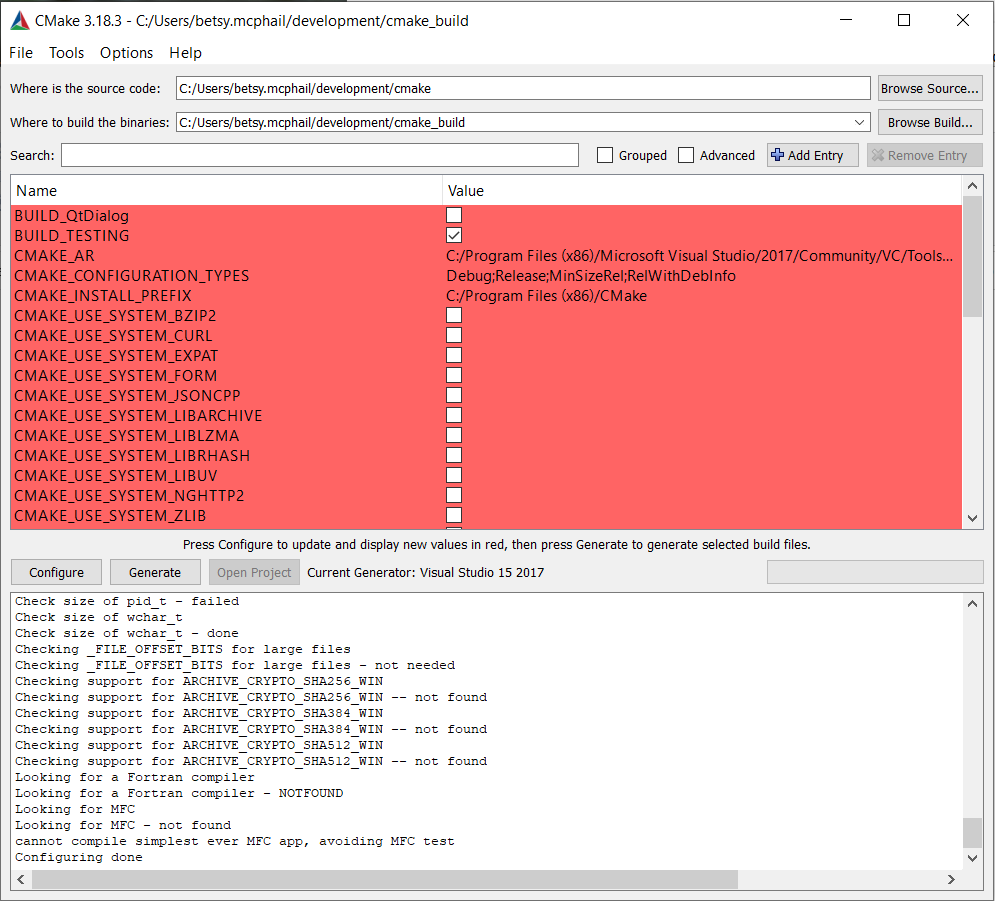
\includegraphics[width=0.66667\linewidth]{cmake-gui}
		    \caption[Tampilan aplikasi cmake-gui]{Tampilan aplikasi cmake-gui.\protect\footnotemark}
		    \label{fig:cmake-gui}
		\end{figure}
		\footnotetext{\href{https://cmake.org/cmake/help/book/mastering-cmake/chapter/Getting\%20Started.html}{https://cmake.org/cmake/help/book/mastering-cmake/chapter/Getting\%20Started.html}}
		
		Dua \textit{field} paling atas adalah direktori dari \textit{source code} dan direktori tempat file-file \textit{binary} nantinya akan diletakkan setelah dibuat. Kedua \textit{field} ini harus diisi secara manual, walaupun jika direktori \textit{binary} ini sudah dikonfigurasi langsung melalui CMake sebelumnya, \textit{field} direktori kedua akan secara otomatis terisi.
		\item ccmake\\
		Di mayoritas sistem operasi berbasis UNIX, jika \textit{library curses}	didukung, maka CMake \linebreak memiliki sebuah perangkat lunak lain yang dapat digunakan, yaitu \verb|ccmake|. Untuk \linebreak menjalankan \verb|ccmake|, pengguna dapat menjalankannya melalui \textit{command line}, dan direktori tempat \verb|ccmake| dijalankan ini harus merupakan direktori tempat file-file \textit{binary} nantinya ingin disimpan. Ketika aplikasi ini dijalankan, akan keluar tampilan seperti di gambar \ref{fig:cmake-ccmake}. Adapun instruksi singkat penggunaan dari aplikasi ini dapat dilihat di bagian bawah dari tampilan tersebut.
		
		\begin{figure}[ht]
		    \centering
		    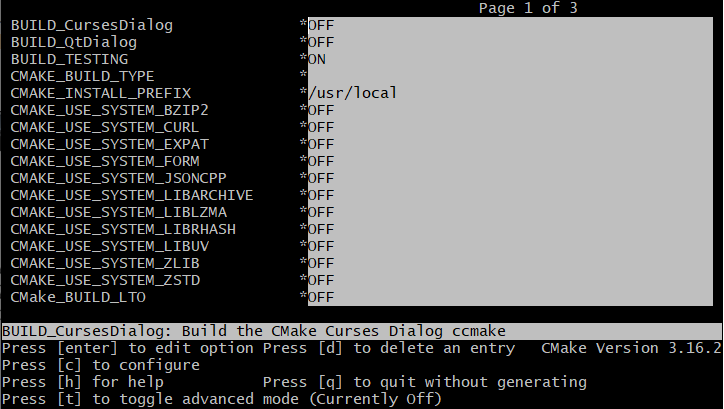
\includegraphics[width=0.66667\linewidth]{cmake-ccmake}
		    \caption[Tampilan aplikasi ccmake]{Tampilan aplikasi ccmake.\protect\footnotemark}
		    \label{fig:cmake-ccmake}
		\end{figure}
		\footnotetext{\href{https://cmake.org/cmake/help/book/mastering-cmake/chapter/Getting\%20Started.html}{https://cmake.org/cmake/help/book/mastering-cmake/chapter/Getting\%20Started.html}}
		
		\item Langsung dari \cl\\
		CMake juga dapat dijalankan melalui \textit{command line}. Untuk menjalankan CMake dari \linebreak \textit{command line}, direktori tempat terminal berada lagi-lagi harus diatur ke direktori tempat file-file \textit{binary} akan disimpan. Kemudian jalankan perintah \verb|cmake| dengan opsi \verb|-D|, \mbox{diikuti} dengan direktori tempat \textit{source code} dari perangkat lunak yang ingin dibangun berada. Walaupun begitu, perlu diingat bahwa metode ini direkomendasikan untuk digunakan hanya untuk proyek-proyek yang memiliki sedikit, atau bahkan tidak ada opsi sama sekali.
	\end{itemize}
	
	\item Pengguna membangun proyek tersebut dengan perkakas pembangunan masing-masing.\\
	CMake dapat memberikan beberapa opsi dalam pembangunan perangkat lunak yang dapat diatur oleh penggunanya masing-masing. Adapun dua opsi utama dari seluruh opsi-opsi tersebut adalah sebagai berikut.
	
	\begin{itemize}
		\item Menspesifikasikan \textit{compiler} yang akan digunakan\\
		Di beberapa sistem, bisa jadi terdapat lebih dari satu \textit{compiler}, atau \textit{compiler} yang ada tidak berada di tempat \textit{compiler} tersebut biasa diinstal. Di kasus-kasus ini, CMake perlu diberitahu secara manual dimana letak \textit{compiler} yang ingin digunakan. Ada tiga cara untuk melakukan ini, yaitu dengan:
		
		\begin{itemize}
			\item menspesifikasikan \textit{compiler} yang ingin dipakai ke generator,
			\item mengatur variabel \textit{environment}, atau
			\item membuat entri \textit{cache}.
		\end{itemize}
		
		Jika pengaturan \textit{compiler} sudah selesai dan \verb|cmake| sudah dijalankan setidaknya sekali, jika pengguna ingin mengganti \textit{compiler}, pengguna harus memulai ulang dengan folder file \textit{binary} yang kosong.
		\item Mengatur konfigurasi pembangunan perangkat\\
		Konfigurasi pembangunan perangkat memungkinkan sebuah proyek untuk dibangun dalam beberapa cara dengan tujuan \textit{debugging}, optimisasi, atau tujuan-tujuan sejenis lainnya. \linebreak Secara \textit{default}, CMake mendukung mode-mode berikut:
		
		\begin{itemize}
			\item \verb|Debug|\textemdash Opsi-opsi \textit{debug} dasar dinyalakan.
			\item \verb|Release|\textemdash Fungsi optimisasi dasar dinyalakan.
			\item \verb|MinSizeRel|\textemdash Ukuran kode akhir diusahakan sekecil mungkin.
			\item \verb|RelWithDebinfo|\textemdash Membangun \textit{build} optimal dan mengikutkan informasi-informasi \linebreak untuk \textit{debugging}.
		\end{itemize}
		
		Dengan generator-generator berbasis Makefile, hanya sebuah mode konfigurasi yang bisa aktif ketika CMake sedang dijalankan, dan mode tersebut diatur dengan variabel \verb|CMAKE_BUILD_| \linebreak \verb|TYPE|. Jika variabel ini dikosongkan (atau tidak dimasukkan ke dalam kode), maka mode yang dipakai adalah mode \textit{default}. Di lain kasus, jika pengembang ingin membangun perangkat dalam dua mode yang berbeda, perintah untuk menjalankan CMake (dengan variabel mode konfigurasi masing-masing) harus dijalankan untuk setiap modenya. 
		Misal, jika pengguna ingin membangun perangkat dengan mode \verb|Debug| dan \verb|Release| sekaligus, maka perintah untuk menjalankan CMake harus ditulis seperti dapat dilihat di potongan kode \ref{code:cmake-multibuild}.
		
		\begin{lstlisting}[caption=Kode utama operasional CMakeLists, label=code:cmake-multibuild]
ccmake ../<direktori> -DCMAKE_BUILD_TYPE=Debug
ccmake ../<direktori> -DCMAKE_BUILD_TYPE=Release
		\end{lstlisting}
		
	\end{itemize}
	
	Setelah CMake dijalankan, proyek tersebut siap untuk dibangun. Jika generator yang dipilih \linebreak merupakan generator berbasis Makefile, maka proyek tersebut dapat dibangun dengan \linebreak mengganti \textit{working directory} ke lokasi file-file \textit{binary}, dan kemudian menjalankan perintah \verb|make|. Jika generator yang dipilih merupakan sebuah IDE, maka proyek tersebut dapat dibangun secara biasa melalui IDE tersebut.
\end{enumerate}
		
		\item \textbf{Membangun perangkat lunak berdasarkan rancangan yang sudah dibuat, dengan \linebreak mengimplementasikan seluruh modul dan \textit{library} yang telah ditentukan di tahap sebelumnya dalam bahasa C.}\\
		{\bf Status :} Ada sejak rencana kerja skripsi.\\
		{\bf Hasil :} Poin ini akan dikerjakan di Skripsi 2.

		\item \textbf{Melakukan pengujian fungsional dan perbaikan \textit{bug}.}\\
		{\bf Status :} Ada sejak rencana kerja skripsi.\\
		{\bf Hasil :} Poin ini akan dikerjakan di Skripsi 2.
		
% Example of dropped step
%		\item \textbf{Melakukan pengujian fungsional dan perbaikan \textit{bug}.}\\
%		{\bf Status :} Tidak dikerjakan \\
%		{\bf Hasil :} Berdasarkan analisis singkat, tidak dilakukan analisis lebih jauh karena tidak diperlukan struktur data baru, karena sudah disediakan oleh OpenSteer versi terbaru

		\item \textbf{Menulis dokumentasi perangkat lunak.}\\
		{\bf Status :} Ada sejak rencana kerja skripsi.\\
		{\bf Hasil :} Poin ini akan dikerjakan di Skripsi 2.

		\item \textbf{Menulis dokumen skripsi.}\\
		{\bf Status :} Ada sejak rencana kerja skripsi.\\
		{\bf Hasil :} Dokumen skripsi akan ditulis hingga bab 3 pada Skripsi 1. Pengisian sisa dari dokumen skripsi, serta penyempurnaan bab 1 sampai bab 3, akan dilakukan pada Skripsi 2.

	\end{enumerate}

\section{Pencapaian Rencana Kerja}
\label{sec:progress}
Langkah-langkah kerja yang berhasil diselesaikan dalam Skripsi 1 ini adalah sebagai berikut:

\begin{enumerate}
	\item Melakukan eksplorasi fungsi-fungsi perangkat lunak KIRI serta eksplorasi cara implementasi API KIRI.
	\item Mempelajari perkakas-perkakas \cl sejenis.
	\item Mempelajari bahasa pemrograman C serta mempelajari dokumentasi-dokumentasi dari seluruh modul yang dibutuhkan untuk pembuatan perangkat lunak.
	\item Melakukan analisis dan desain perangkat lunak yang akan dibangun.
	\item Melakukan analisis kebutuhan fitur-fitur perangkat lunak. (Tidak dilakukan)
	\item Melakukan eksplorasi \textit{library} yang dapat digunakan.
	\item[10.] Menulis dokumen skripsi. (Hanya sampai bab 3)
\end{enumerate}

%TULISKAN BAGIAN INI JIKA DOKUMEN ANDA TIPE A ATAU C
\begin{comment}
	\section{Kendala yang Dihadapi}
	Kendala - kendala yang dihadapi selama mengerjakan skripsi :
	\begin{itemize}
		\item Terlalu banyak melakukan prokrastinasi.
		\item Terlalu banyak godaan berupa hiburan (game, film, dll)
		\item Skripsi diambil bersamaan dengan kuliah ASD karena selama 5 semester pertama kuliah tersebut sangat dihindari dan tidak diambil, dan selama 4 semester terakhir kuliah tersebut selalu mendapat nilai E
		\item Mengalami kesulitan pada saat sudah mulai membuat program komputer karena selama ini selalu dibantu teman
	\end{itemize}
\end{comment}

\bibliographystyle{compj}
\bibliography{referensi} 

\vspace{3cm}
\centering Jakarta, \tanggal\\
\vspace{2cm} \nama \\ 
\vspace{1cm}

Menyetujui, \\
\ifdefstring{\jumpemb}{2}{
\vspace{1.5cm}
\begin{centering} Menyetujui,\\ \end{centering} \vspace{0.75cm}
\begin{minipage}[b]{0.45\linewidth}
% \centering Bandung, \makebox[0.5cm]{\hrulefill}/\makebox[0.5cm]{\hrulefill}/2013 \\
\vspace{2cm} Nama: \pembA \\ Pembimbing Utama
\end{minipage} \hspace{0.5cm}
\begin{minipage}[b]{0.45\linewidth}
% \centering Bandung, \makebox[0.5cm]{\hrulefill}/\makebox[0.5cm]{\hrulefill}/2013\\
\vspace{2cm} Nama: \pembB \\ Pembimbing Pendamping
\end{minipage}
\vspace{0.5cm}
}{
% \centering Bandung, \makebox[0.5cm]{\hrulefill}/\makebox[0.5cm]{\hrulefill}/2013\\
\vspace{2cm} Nama: \pembA \\ Pembimbing Tunggal
}
\end{document}

